\documentclass[a4paper]{article}

\usepackage[english]{babel}
\usepackage{multirow}
\usepackage{caption} 
\captionsetup[table]{skip=10pt}
\usepackage[utf8x]{inputenc}
\usepackage[T1]{fontenc}
\usepackage{pdfpages}
\usepackage{nomencl}
\makenomenclature
\renewcommand{\nomname}{List of Symbols}
\renewcommand{\abstractname}{Summary}
\usepackage{amsmath}
\usepackage{acro}
\usepackage{listings}
\usepackage{color}
\definecolor{codegreen}{rgb}{0,0.6,0}
\definecolor{codegray}{rgb}{0.5,0.5,0.5}
\definecolor{codepurple}{rgb}{0.58,0,0.82}

 \textwidth = 426pt
\lstdefinestyle{mystyle}{
    commentstyle=\color{codegreen},
    keywordstyle=\color{magenta},
    stringstyle=\color{codepurple},
    basicstyle=\footnotesize,
    breakatwhitespace=false,         
    breaklines=true,                 
    captionpos=b,                    
    keepspaces=true,                 
    showspaces=false,                
    showstringspaces=false,
    showtabs=false,                  
    tabsize=2
}
 
\lstset{style=mystyle}
% probably a good idea for the nomenclature entries:
\acsetup{first-style=short}
%% Sets page size and margins
\usepackage[a4paper,top=3cm,bottom=2cm,left=3cm,right=3cm,marginparwidth=1.5cm]{geometry}
%% Useful packages
\usepackage{amsmath}
\usepackage[shortlabels]{enumitem}
\usepackage{parskip}
\usepackage{float}
\usepackage{graphicx}
\usepackage{nicefrac} % For comparison
\usepackage{xfrac} 
\usepackage[euler]{textgreek}
\usepackage[colorlinks=true, allcolors=blue]{hyperref}


\title{Design 3 - Mechanism Feasibility Study}
\author{10693, 10926 and 10965}
\date{November 2018}




\clearpage
\begin{document}
\maketitle
\renewcommand{\abstractname}{Summary}

\begin{figure}[H]
\centering
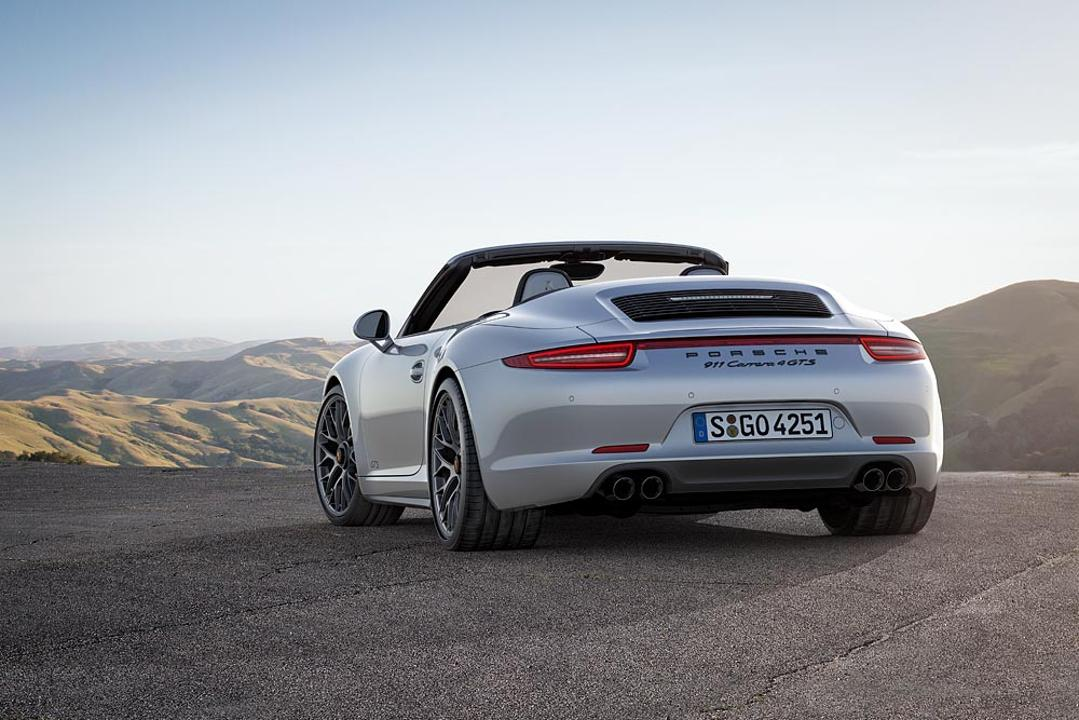
\includegraphics[width=1\textwidth]{Car.jpg}
\caption{911 Carrera 4 GTS Cabriolet, 2014, Porsche AG. \cite{porschenewsroom}}
\end{figure}

\begin{abstract}

This report explores the feasibility of concepts for a Porsche 911 Carrera cabriolet roof mechanism, generated according to requirements outlined in the PDS and compared against each other in order to determine which is most suitable. Initial concepts were generated by researching similar mechanisms and prototypes created to visualise the feasibility and deployment. Concepts were compared using multi-criteria decision analysis and a final concept was selected.  The selected mechanism was modelled and refined in order to perfectly fit the requirements stated in the PDS, Table \ref{PDS}. Different motor, gear ratio and damping coefficient configurations were investigated and compared to obtain suitable values for output torque and speed of rotation. The ideal values for these were then selected  to give a gear ratio of 1800:1 and maximum output torque of 159.2 Nm.  A multi-stage gearbox was designed to transmit the required torque at 1800:1. The gearbox had five stages with ratios of 5:1, 5:1, 4.5:1, 4:1 and 4:1 to give the necessary overall ratio. It was found that the mechanism was a feasible design which created an ideal balance between all of the categories discussed in the PDS. With a damping coefficient of 7 Nm/deg/s the project achieved a suitable working roof mechanism which closed in 13.8 seconds, forming an aesthetic shape.


\end{abstract}
\clearpage


\tableofcontents
\printnomenclature



\section{Introduction}

%Mechanisms form an important part of the design of dynamic mechanical systems and convertible roof deployment is a common example of their use. 
In this task a design brief was set to design a mechanism and accompanying motor and gearbox to deploy a convertible roof for a Porsche 911 Carrera. This luxury addition to the car reignites the thrill for many drivers and the freedom of feeling the wind rushing past while still retaining the practicality of having a roof when it is needed. The mechanism was intended to fit into an area on the side profile of 580 mm x 295 mm when in the retracted position and extend to the top of windscreen, a distance of 1550 mm x 445 mm from the rearmost point of the storage area. A concept of the mechanism was to be modelled within Simulink and a motor, overall gear ratio and damping coefficient were to be selected to deploy the mechanism safely and in a reasonable time. A multi-stage gearbox for the motor was then to be designed with appropriate steps to produce the overall gear ratio and transfer the motor torque to the mechanism.

\section{Design Specification}

The product design specification (PDS) was primarily formed using the design brief, EU legislation \cite{UN/ECE} and the course notes \cite{Coursenotes}. An initial draft was produced before the design work began but the PDS continued to be amended throughout the design process as design constraints were found and further criteria were raised.

\begin{table}[H]
\centering \caption{\label{PDS} Product Design Specification}
\hspace*{-1.5cm}\begin{tabular}{||c|c|c|c|c|c||}
\hline
Category & No & Date & Requirement & Must/Wish & Method of Evaluation \\ \hline\hline
\multirow{4}{*}{Performance} & 1 & 6/11/2018 & \begin{tabular}[c]{@{}c@{}}Minimum of 2 mounting points\\ for fabric roof on mechanism\end{tabular} & Must & Simulink Model \\ \cline{2-6} 
 & 2 & 7/11/2018 & \begin{tabular}[c]{@{}c@{}}Total deployment time\\ under 15 seconds\end{tabular} & Wish & Simulink Model \\ \cline{2-6} 
 & 3 & 7/11/2018 & \begin{tabular}[c]{@{}c@{}}Minimal torque required\\ for deployment\end{tabular} & Wish & Motor Selection \\ \cline{2-6} 
 & 4 & 12/11/2018 & Mass kept to a minimum & Wish & Concept Selection \\ \hline
\multirow{5}{*}{Features} & 5 & 6/11/2018 & \begin{tabular}[c]{@{}c@{}}Span to Point 1550mm x 445mm from \\ furthest bottom edge of storage space\end{tabular} & Must & Simulink Model \\ \cline{2-6} 
 & 6 & 6/11/2018 & Retract into 295mm x 580mm space & Must & Simulink Model \\ \cline{2-6} 
 & 7 & 6/11/2018 & \begin{tabular}[c]{@{}c@{}}Entire mechanism operated\\ by single motor\end{tabular} & Must & Motor Selection \\ \cline{2-6} 
 & 8 & 26/11/2018 & 12V power supply & Must & Motor Selection  \\ \cline{2-6} 
 & 9 & 26/11/2018 & \begin{tabular}[c]{@{}c@{}}Thickness of roof minimised\\ once deployed\end{tabular} & Wish & Simulink Model \\ \hline
\multirow{5}{*}{Reliability} & 10 & 7/11/2018 & Operate in all weather conditions & Must & Concept Selection \\ \cline{2-6} 
 & 11 & 12/11/2018 & Service interval of 3 years & Wish & Motor Selection \\ \cline{2-6} 
 & 12 & 26/11/2018 & \begin{tabular}[c]{@{}c@{}}Working temperature\\ -25 to 40$^\circ$C\end{tabular} & Must & Motor Selection \\ \cline{2-6} 
 & 13 & 26/11/2018 & Working humidity 0 to 100\% & Must & Motor Selection \\ \hline
\multirow{2}{*}{Conformance} & 14 & 19/11/2018 & \begin{tabular}[c]{@{}c@{}}No infringement\\ of existing patents\end{tabular} & Must & Solution Specification \\ \cline{2-6} 
 & 15 & 19/11/2018 & \begin{tabular}[c]{@{}c@{}}Meets crash safety\\ roll-over legislation\end{tabular} & Must & Solution Specification \\ \hline
\multirow{2}{*}{Durability} & 16 & 6/11/2018 & \begin{tabular}[c]{@{}c@{}}Design life of 18000 cycles (4 cycles \\ per day, 300 days per year, 15 years)\end{tabular} & Must & Motor selection \\ \cline{2-6}
 & 17 & 6/11/2018 & Minimise energy consumption & Wish & Motor selection \\ \hline
Serviceability & 18 & 19/11/2018 & \begin{tabular}[c]{@{}c@{}} Simple mounting to chassis\\ for easy removal\end{tabular} & Wish & Simulink Model \\ \hline
\multirow{2}{*}{Aesthetics} & 19 & 12/11/2018 & \begin{tabular}[c]{@{}c@{}}Uppermost points of the mechanism \\ form a smooth curve\end{tabular} & Wish & Simulink Model \\ \cline{2-6} 
 & 20 & 26/11/2018 & No sudden changes in roof speed & Wish & Simulink Model \\ \cline{2-6} 
 & 21 & 26/11/2018 & Glass window at back of roof & Wish & Concept Selection \\ \hline
\multirow{2}{*}{\begin{tabular}[c]{@{}c@{}}Manufacture\\ \& Assembly\end{tabular}} 
& 22 & 12/11/2018 & \begin{tabular}[c]{@{}c@{}}All links assembled only using\\ rigid or rotating joints\end{tabular} & Must & Simulink Model \\ \cline{2-6} 
 & 23 & 12/11/2018 & \begin{tabular}[c]{@{}c@{}}Mechanism fitted to vehicle\\ as one component\end{tabular} & Must & Simulink Model \\ \hline\hline
\end{tabular}
\end{table}

\section{Concept Design}

To generate concepts of the mechanism, similar mechanisms were first researched and analysed to provide a basis for possible design ideas. These ideas were then used to create three initial concepts. Prototype models of these concepts were then manufactured using craft sticks and pins to help visualise the feasibility of the designs. These physical models were roughly measured and values were compared to approximate ratios of retracted and extended length and height to determine their potential success. Initial Simulink models were created by scaling the physical measurements of the prototypes, using standardised beam and joint dimensions, to approximately fit to the constraints of the design brief specifications. This allowed the practicality of each design to be assessed in relation to the requirements shown in the PDS, table \ref{PDS}.

\begin{figure}[H]
  \centering
  \begin{minipage}[b]{0.3\textwidth}
    \centering
    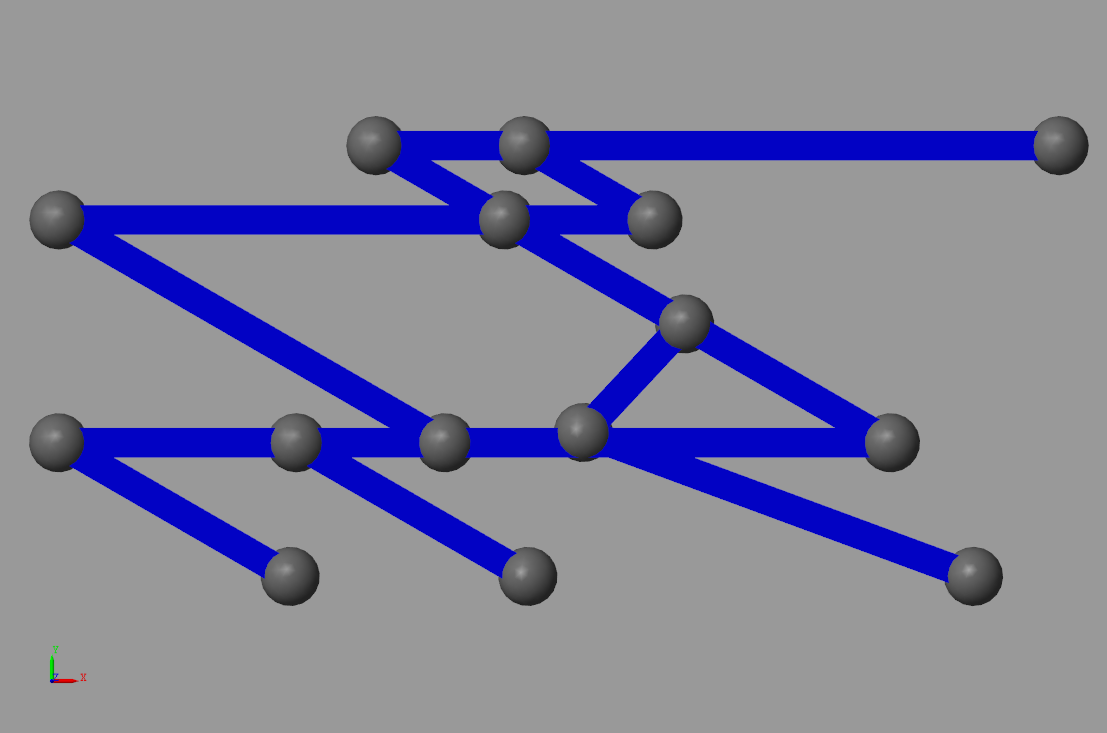
\includegraphics[width=1\textwidth]{Fabian.PNG}
    \caption{\label{conceptA} Simulink model of Concept A}
  \end{minipage}
  \hfill
  \begin{minipage}[b]{0.3\textwidth}
    \centering
    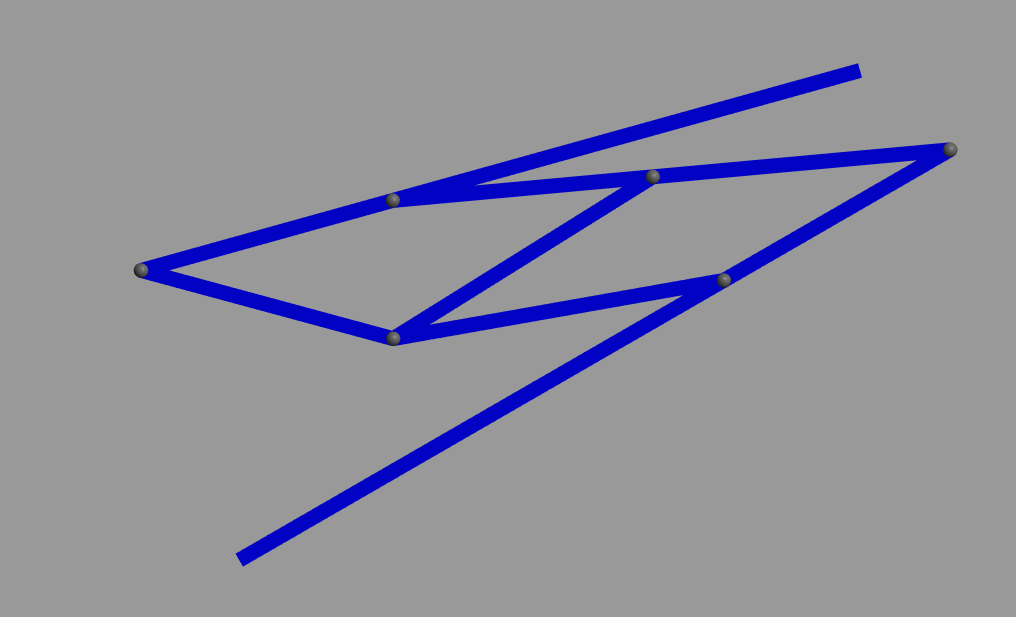
\includegraphics[width=1\textwidth]{Terry.PNG}
    \caption{\label{conceptB} Simulink model of Concept B}
  \end{minipage}
  \hfill
   \begin{minipage}[b]{0.3\textwidth}
     \centering
    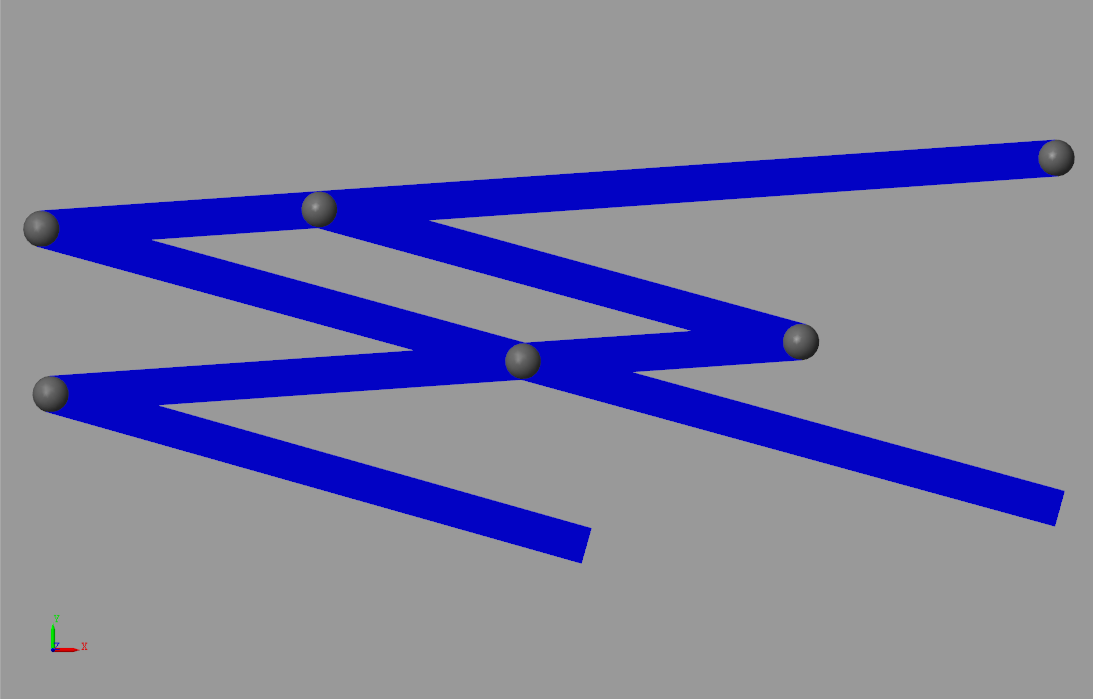
\includegraphics[width=1\textwidth]{Stuart.PNG}
    \centering
    \caption{\label{conceptC} Simulink model of Concept C}
  \end{minipage}
\end{figure}

\paragraph{}
Concept A, shown in the retracted position in Figure \ref{conceptA}, was driven from the bottom right joint in the model. Whilst Concept A appeared to function at the initial design stage, it was unable to be deployed to full length within Simulink, even after modifications were made, as the model was found to be too top heavy and therefore collapsed into itself. In the retracted position, the model fit into the storage space available however the length of the deployed position could not be determined using Simulink. The holding torque for Concept A could not be determined from the Simulink model due to the aforementioned problems.

\paragraph{}
Concept B, shown in the retracted position in Figure \ref{conceptB},  was driven from the first joint on the lower support beam; the motor rotates the driving beam to the deployed position as shown in figure \ref{DeployedB}. Concept B retracted into the space specified however, in deployment, the model was unable to reach the distance required by the length of the car. The torque required to hold the model in the starting position was calculated using Simulink and was found to be 21.45 Nm. 

\paragraph{}
Concept C, shown in the retracted position in Figure \ref{conceptC}, was driven from the right hand ground joint in the model; the motor rotates the mechanism about the point to the deployment position shown in Figure \ref{DeployedC}. The model was able to fit within the specified storage space and was deployed to the distance required to reach the windscreen. The holding torque for the model in the initial position was determined to be 18.05 Nm.

\begin{figure}[H]
    \centering
\begin{minipage}[b]{0.4\textwidth}
    \centering
    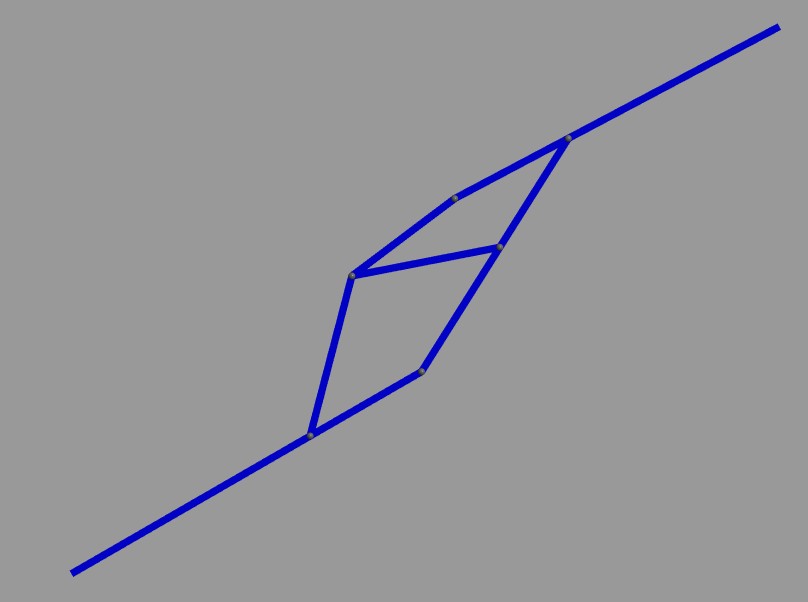
\includegraphics[width=1\textwidth]{TerryDep.PNG}
    \caption{\label{DeployedB} Simulink model of Concept B Deployed}
  \end{minipage}
\hfill
   \begin{minipage}[b]{0.4\textwidth}
     \centering
    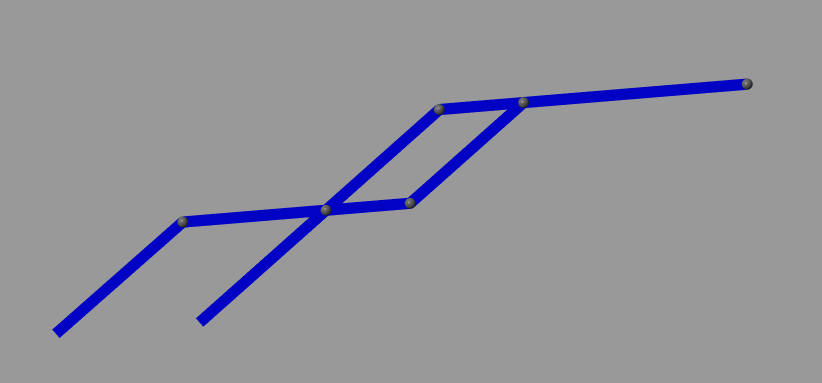
\includegraphics[width=1\textwidth]{StuartDep.PNG}
    \centering
    \caption{\label{DeployedC} Simulink model of Concept C Deployed}
  \end{minipage}
\end{figure}

\section{Concept Selection}
The concepts were scored using mechanism multi-criteria decision analysis (MCDA), where each concept was scored against requirements which the final design aimed to meet. Each requirement was given a weighting relative to its importance for the design and a total score for each concept was calculated, as seen in Figure \ref{MCDA}. These weightings were calculated by comparing each criteria to the others and ordering their importance seen in Table \ref{PWC}

\begin{table}[H]
\caption{Pair-wise comparison for weighting requirements}
\label{PWC}
\begin{tabular}{||l|l||l|l|l|l|l|l|l||}
\hline
Function &  & \multicolumn{1}{l|}{A} & \multicolumn{1}{l|}{B} & \multicolumn{1}{l|}{C} & \multicolumn{1}{l|}{D} & \multicolumn{1}{l|}{E} & \multicolumn{1}{l|}{F} & G \\ \hline\hline
Manufacturing Complexity & A & - & A & C & A D & E & F & G \\ \cline{1-2}
Mass & B & - & - & C & D & E & F & G \\ \cline{1-2}
Conformance with Dimensional Constraints & C & - & - & - & C & E & F C & G \\ \cline{1-2}
Deployment Time & D & - & - & - & - & E & F & G \\ \cline{1-2}
Roof Form Aesthetic & E & - & - & - & - & - & E & G \\ \cline{1-2}
Potential Failure & F & - & - & - & - & - & - & G \\ \cline{1-2}
Torque Required for Operation & G & - & - & - & - & - & - & - \\ \hline\hline
\end{tabular}
\end{table}

\paragraph{}
Concept A had an extremely complex and heavy design which failed upon testing within Simulink. It fit within the dimensional constraints however could not be deployed from this position. Considering the initial prototype, the deployed position formed a reasonably aesthetic shape but there was not enough time to develop the prototype in Simulink to analyse deployment.

\paragraph{}
Concept B had a simple design which was light and did not easily fail. It fit within the storage parameters and deployed quickly with a relatively low torque (standardised torque of 21.45 Nm) however was unable to reach the required distance. It formed a very arched roof form.

\paragraph{}
Concept C had a relatively simple design with low potential failure and low mass. It fit easily within the constraints and deployed quickly using a low torque (standardised torque of 18.05 Nm) to form an aesthetic spacious roof form. 

\begin{table}[H]
\caption{Mechanism Multi-criteria Decision Analysis}
\label{MCDA}
\hspace*{-0.75cm}\begin{tabular}{||l|l|l|l|l|l|l|l||}
\hline
 &  & \multicolumn{2}{l|}{Concept C} & \multicolumn{2}{l|}{Concept A} & \multicolumn{2}{l|}{Concept B} \\ \hline
Criteria & Weighting & Score & Weighted & Score & Weighted & Score & Weighted \\ \hline\hline
\begin{tabular}[c]{@{}l@{}}Manufacturing \\ Complexity\end{tabular} & 6 & 8 & 48 & 3 & 18 & 7 & 42 \\ \hline
Mass & 4 & 7 & 28 & 4 & 16 & 7 & 28 \\ \hline
\begin{tabular}[c]{@{}l@{}}Conformance with \\ Dimensional Constraints\end{tabular} & 8 & 9 & 72 & 4 & 32 & 5 & 40 \\ \hline
Deployment Time & 6 & 8 & 48 & 3 & 18 & 7 & 42 \\ \hline
Roof Form Aesthetic & 9 & 8 & 72 & 7 & 63 & 4 & 36 \\ \hline
Potential Failure & 8 & 8 & 64 & 2 & 16 & 8 & 64 \\ \hline
\begin{tabular}[c]{@{}l@{}}Torque Required\\ for Operation\end{tabular} & 10 & 8 & 80 & 0 & 10 & 7 & 70 \\ \hline
Total &  &  & 510 &  & 510 &  & 510 \\ \hline
\% of Total &  &  & 80.78 &  & 33.92 &  & 63.14 \\ \hline
Rank &  &  & 1 &  & 3 &  & 2 \\ \hline\hline
\end{tabular}
\end{table}

After assessing the concepts using the MCDA (Table \ref{MCDA}) it was found that Concept C was the most suitable mechanism to use as it was the highest scoring and hence was chosen to be carried forward.

\section{Deployment Modelling}
The deployment of the final concept was modelled using Simulink. This allowed the deployment of the mechanism to be visualised more accurately than during the prototyping stage and hence the feasibility of the design to be better assessed. The dimensions and masses of the beams and joints in the mechanism were altered at this stage to better represent the final design. Therefore, in this exercise the mass of the roof material and rear window was distributed over the mechanism to produce a more accurate model. Simulink was first used to calculate the holding torque, which has to be overcome to deploy the model. When a feedback loop and stop simulation are added to the model, the deployment time of the model to the final position can be found. Data for the output position, speed, acceleration and torque of the model can be imported into MATLAB for plotting graphs and further analysis. The fourth-order Runge-Kutta method was chosen as the solver for the model with a fixed time step of 0.001 seconds. The method works by finding a weighted average of the derivatives of the ODE over the time interval, whereas the Euler method assumes the same value across the interval. Therefore the Runge-Kutta method is more accurate in finding solutions as the numerical error at each iteration is reduced.

\paragraph{}
Calculations on the dimensions of Concept C found that the angle of the main diagonal when fully deployed was 45.1$^\circ$. From this angle the forward extension of the main diagonal was calculated at 423.5mm, giving a total extension across the top beam of 546.5mm. This allowed the horizontal extension of the forward most extending bar to be calculated at 397mm. Calculations on the retracted dimensions showed that the front pivot point could be raised by 20mm and hence the angle of incline of the entire assembly was then found to be 4.5$^\circ$. Given this incline, the length of this forward-most beam was found to be 398.2mm. Finally the height due to the angle of this beam was compensated for by reducing the height of the upper parallelogram by 31.2mm.

\paragraph{}
The mass of the rear window was calculated as $5.5 kg$. For this it was assumed that the window had an area of 0.5 m$^2$, a thickness of 5 $mm$. and a density of 2200 $kg/m^3$ \cite{Encyclopaedia}. The mass of the roof material was calculated as 17 kg, assuming an area 1.92 $m^2$, eight layers of (1mm thick, 1.4 $\times 10^3 kg/m^3$ \cite{Canvas}) canvas and one layer of (2mm thick, 900 $kg/m^3$ \cite{CambMaterials}) butyl rubber. The mass of the crossbraces were calculated as 1.1 $kg$ with an extra  0.1 $kg$ assumed for the weight of bearings and other fixtures. In total this gave a roof weight weight of 38.9 $kg$. When the concept was modelled in Simulink, the weight of the roof and window was assumed to act as point masses distributed evenly across each of the relative support points on the mechanism.


\section{Motor, Gear Ratio and Damping Selection}
The motor selection began by assuming an approximate undamped deployment time of 10 seconds, which would allow for extra time once damping was added to the system later in the design development. From this time a target value for gearbox output rotational speed was determined by calculating the total angle through which the driving link of the mechanism needed to rotate, and hence calculating the target rotational speed from this. The holding torque of the mechanism when retracted was also carried forward to this section of the development to act as a minimum value for stall torque for the output of the gearbox.

\begin{table}[H]
\centering
\caption{Idealised Target Values for Gearbox Output}
\label{Target}
\begin{tabular}{||l|l||}
\hline
Output Speed (rad/s) & 0.20943951 \\ \hline
Output Stall Torque (Nm) & 159.2 \\ \hline\hline
\end{tabular}
\end{table}

\paragraph{}
Using these values an initial assessment of potential motors was undertaken. The stall torque, nominal torque and rotational speed at the nominal torque were recorded for each motor from the manufacturer data and placed into a table. The rotational speed for each was then converted from the manufacturer quoted values in rpm into rad/s. The target value of gearbox output rotational speed was then used to find a gear ratio for each motor that would allow the output to match the target. From this, the output stall torque and nominal torque for each was calculated.

\begin{table}[H]
\centering
\caption{Initial Motor Assessment}
\label{IMA}
\hspace*{-2cm}\begin{tabular}{|l|l|l|l|l|l|l|l|l|}
\hline
\begin{tabular}[c]{@{}l@{}}Motor Part\\ Number\end{tabular} & \begin{tabular}[c]{@{}l@{}}Stall \\ Torque \\ (Nm)\end{tabular} & \begin{tabular}[c]{@{}l@{}}Nominal \\ Torque \\ (Nm)\end{tabular} & \begin{tabular}[c]{@{}l@{}}Motor Speed \\ at Nominal \\ Torque (rpm)\end{tabular} & \begin{tabular}[c]{@{}l@{}}Motor Speed \\ at Nominal \\ Torque (rad/s)\end{tabular} & \begin{tabular}[c]{@{}l@{}}Gear \\ Ratio \end{tabular} & \begin{tabular}[c]{@{}l@{}}Output \\ Stall \\ Torque\end{tabular} & \begin{tabular}[c]{@{}l@{}}Output \\ Nominal \\ Torque (Nm)\end{tabular} & \begin{tabular}[c]{@{}l@{}}Output Nominal\\ Speed (rad/s)\end{tabular} \\ \hline
0 130 001 001 & 0.19 & 0.04 & 4000 & 418.8790205 & 2000 & 380 & 80 & 0.20943951 \\ \hline
0 390 204 092 & 0.43 & 0.05 & 2400 & 251.3274123 & 1200 & 516 & 60 & 0.20943951 \\ \hline
0 390 204 118 & 0.48 & 0.05 & 7200 & 753.9822369 & 3600 & 1728 & 180 & 0.20943951 \\ \hline
0 390 204 166 & 0.69 & 0.028 & 3550 & 371.7551307 & 1775 & 1224.75 & 49.7 & 0.20943951 \\ \hline
\end{tabular}
\end{table}

\paragraph{}
Following this initial assessment it was realised that all the motors greatly exceeded the minimum requirements for stall torque and hence the smallest motor was chosen as the motor that would be carried through into further development. It can be seen from Figure \ref{Mspeed} and the Black line in Figure \ref{Mstat} that the operating speeds for deployment are suitable for the selected motor.

\begin{figure}[H]
 \centering
\begin{minipage}[b]{0.4\textwidth}
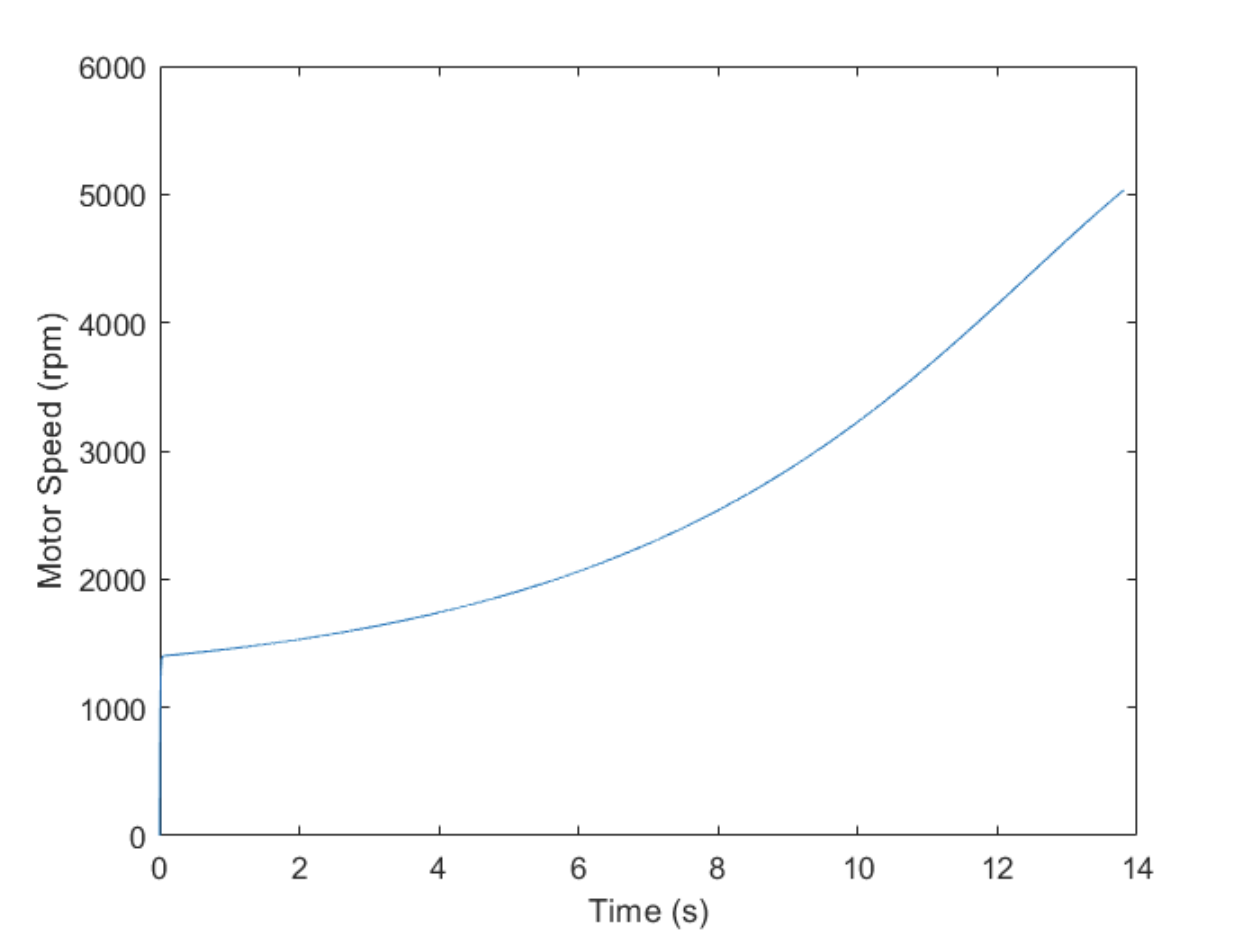
\includegraphics[width=1\textwidth]{MotorSpeed.png}
    \caption{\label{Mspeed} Graph showing the rotational speed of the motor during deployment}
\end{minipage}
\hfill
\begin{minipage}[b]{0.4\textwidth}
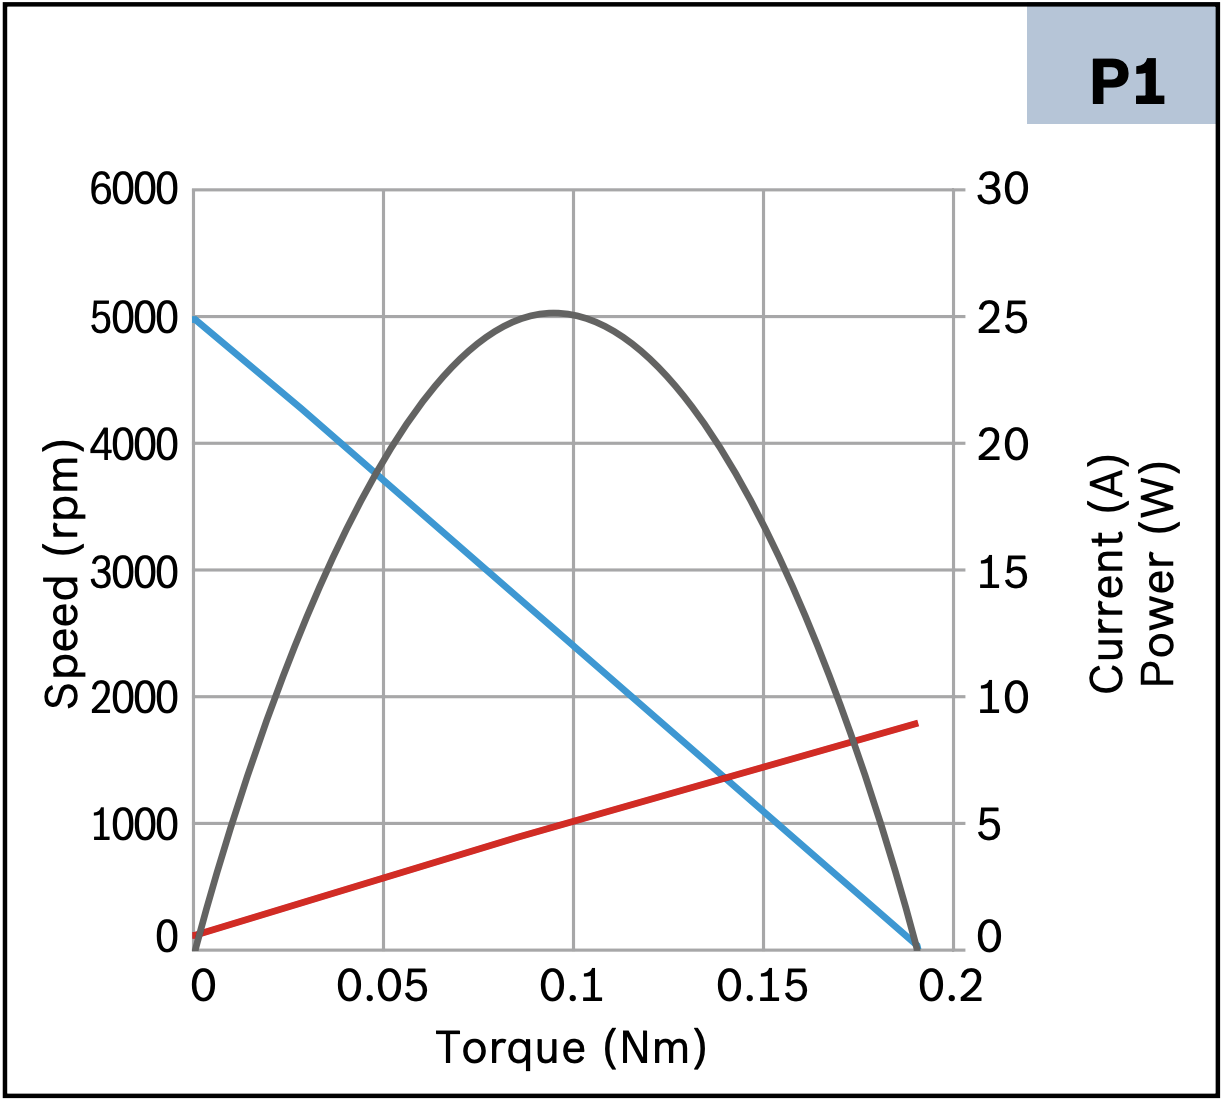
\includegraphics[width=0.9\textwidth]{Motorstat.png}
    \caption{\label{Mstat} Graph showing suitable motor speeds}
\end{minipage}
\end{figure}

\paragraph{}
A feedback loop to drive the Simulink model was then created to represent the behaviour of the motor and gearbox. The first step was to calculate the motor function, which would allow the torque produced by the motor to be calculated from the current motor speed at each step of the solver. This was done by considering the linear relationship between speed and torque for DC motors and using the manufacturer supplied data for the motor. The gradient of the line was found using the nominal and stall torque values and from this a value for the no-load speed of the motor was calculated. This allowed the equation of the line to be found and rearranged to give the torque value for a given speed.


This motor function was incorporated into the wider feedback loop, which used the output of the speed of the driving joint. This value was first converted from rad/s into rpm then used to calculate the motor speed by multiplying by the gear ratio. This value was then passed through the motor function to give the motor torque and again multiplied by the gear ratio to give the gearbox output torque.


Initial testing was then performed to assess whether the use of a gear ratio significantly different to that calculated at the initial motor assessment stage would produce a significantly faster deployment time and was found not to be the case.


A nominal value of 4 Nm/deg/s was chosen as the initial value for rotational damping coefficient. The characteristic response of the system for different configurations of gear and damping coefficient was then assessed by keeping the damping coefficient constant whilst changing the gear ratio from 1800:1 to 2200:1 and recording angle, torque, power and angular speed of the driven joint at each time step of the simulation. This process was then repeated for rotational damping coefficient values of 5, 6 \& 7 Nm/deg/s, and the results for each damping coefficient are shown in Figures \ref{Damping4}, \ref{Damping5}, \ref{Damping6} \& \ref{Damping7}.


\begin{figure}[H]
\centering
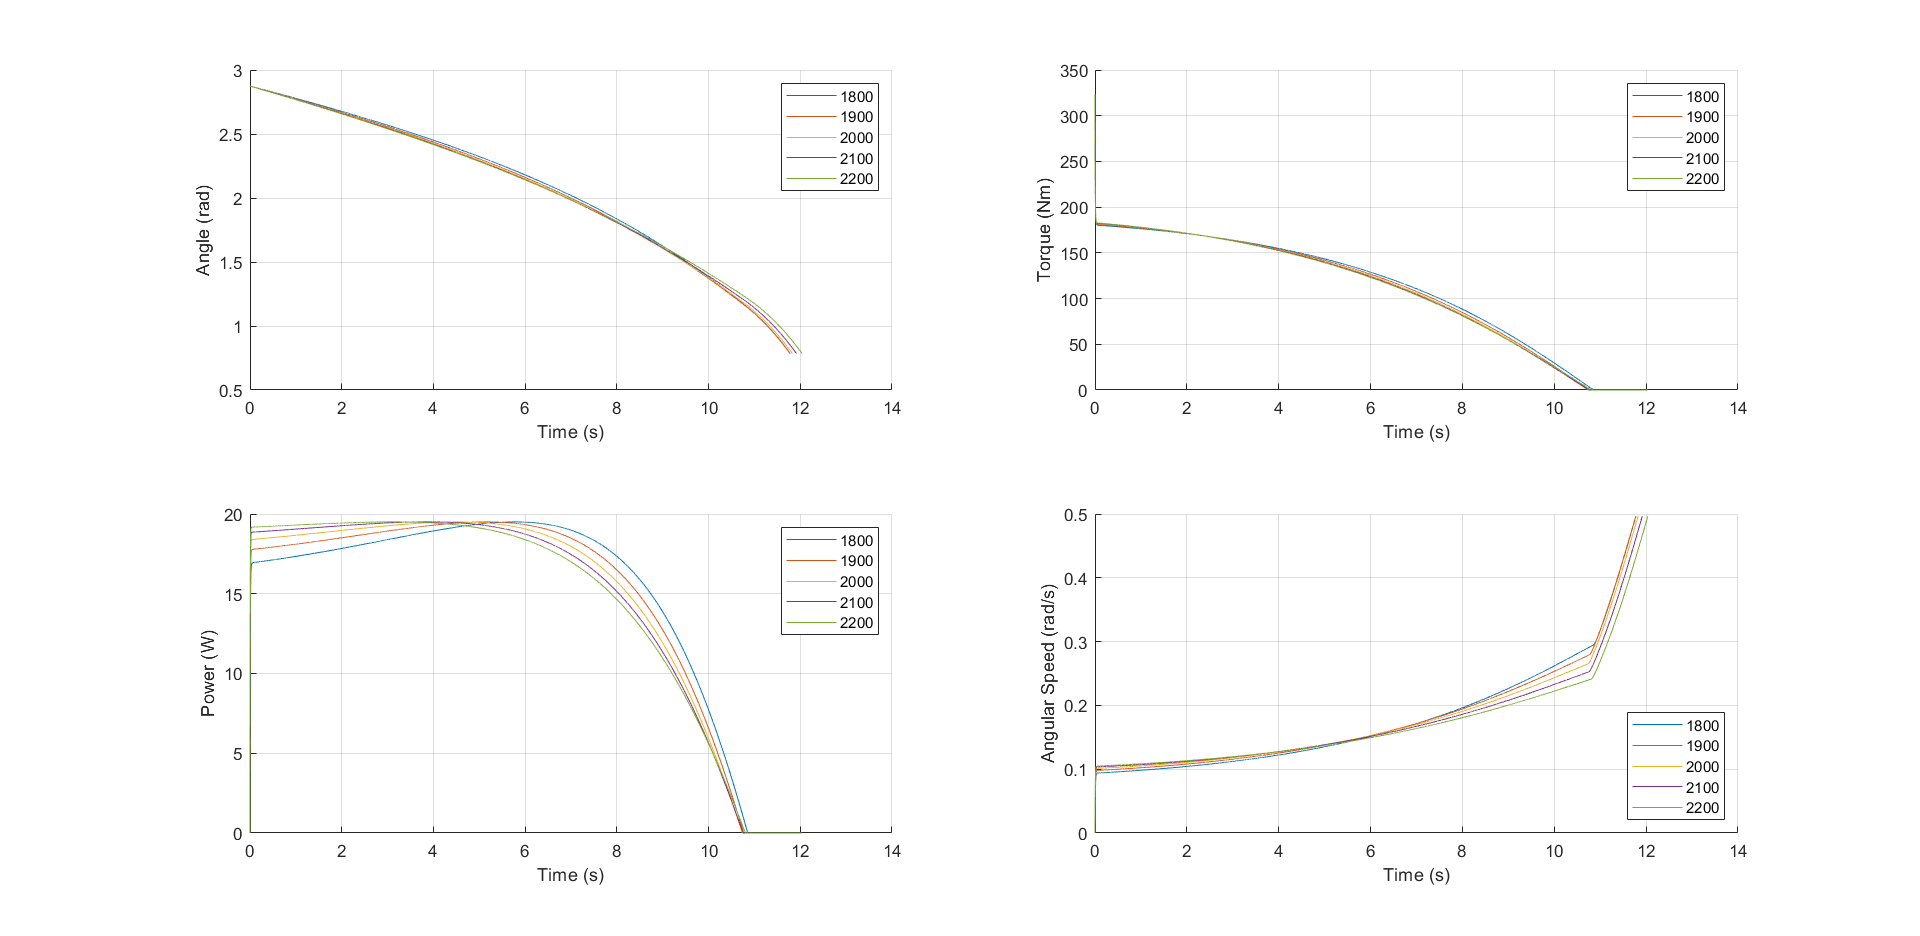
\includegraphics[width=1\textwidth]{Damping_4.png}
    \caption{\label{Damping4} Graphs with damping coefficient of 4}
\end{figure}

\begin{figure}[H]
\centering
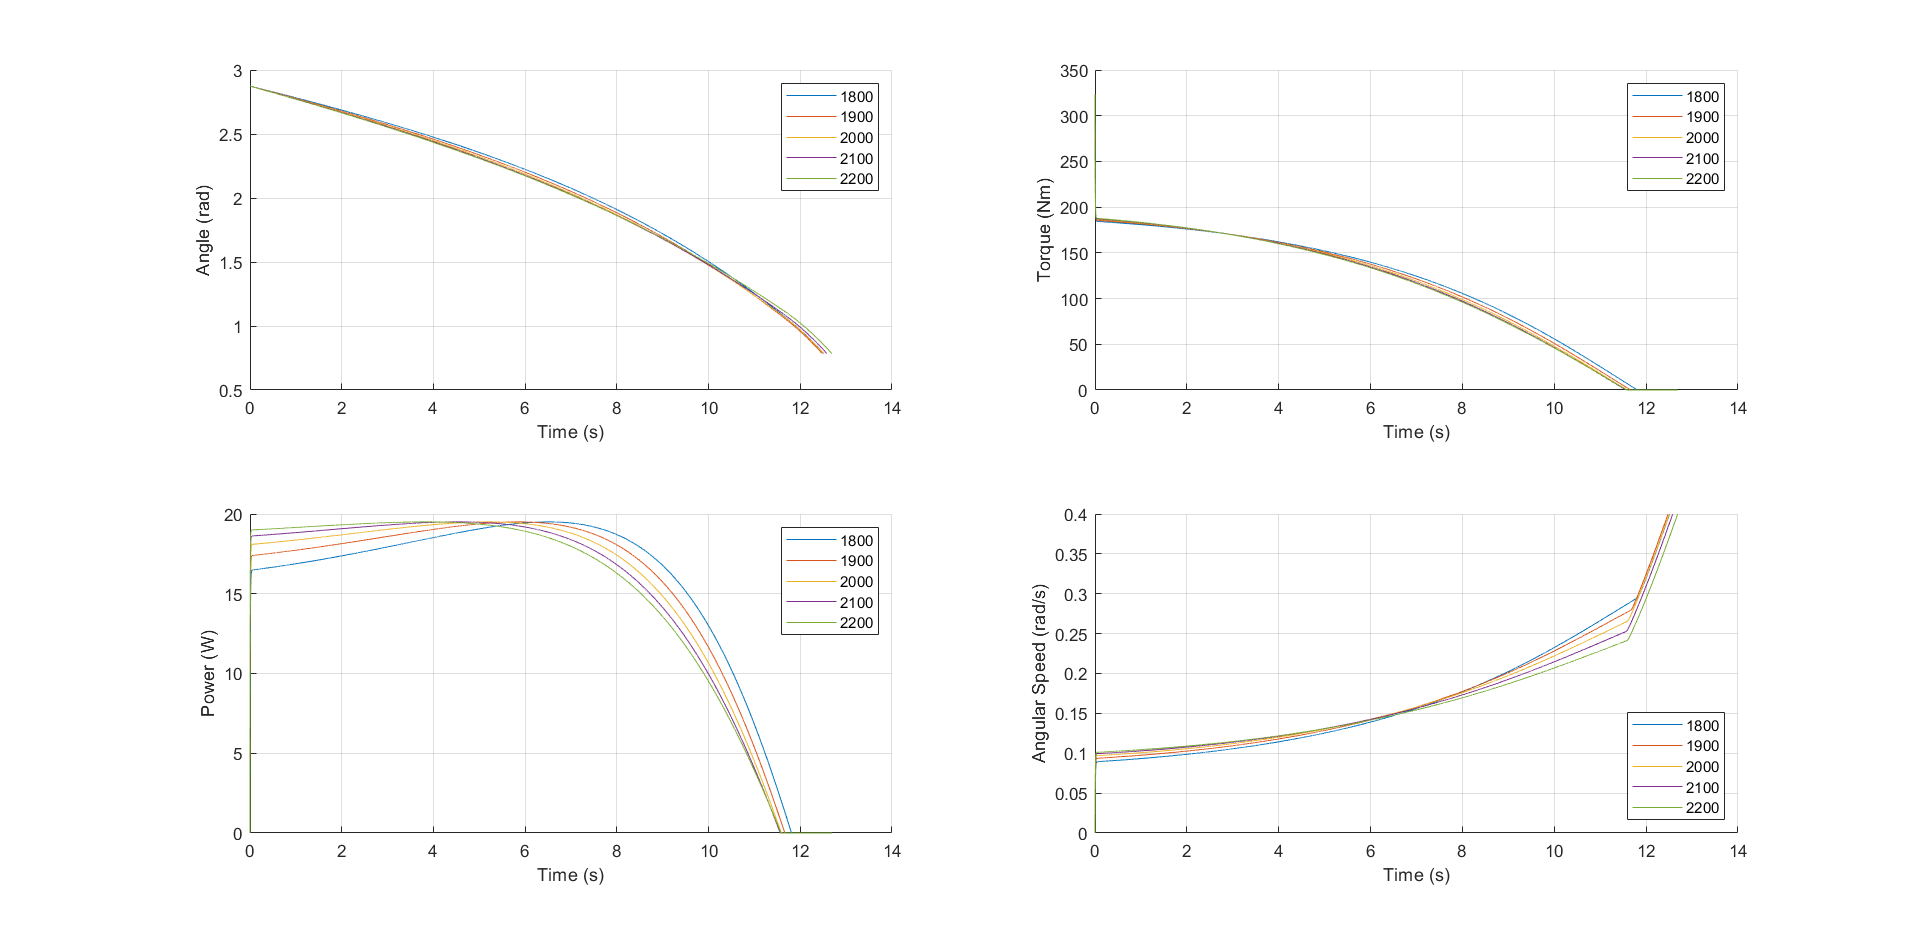
\includegraphics[width=1\textwidth]{Damping_5.png}
    \caption{\label{Damping5} Graphs with damping coefficient of 5}
\end{figure}

\begin{figure}[H]
\centering
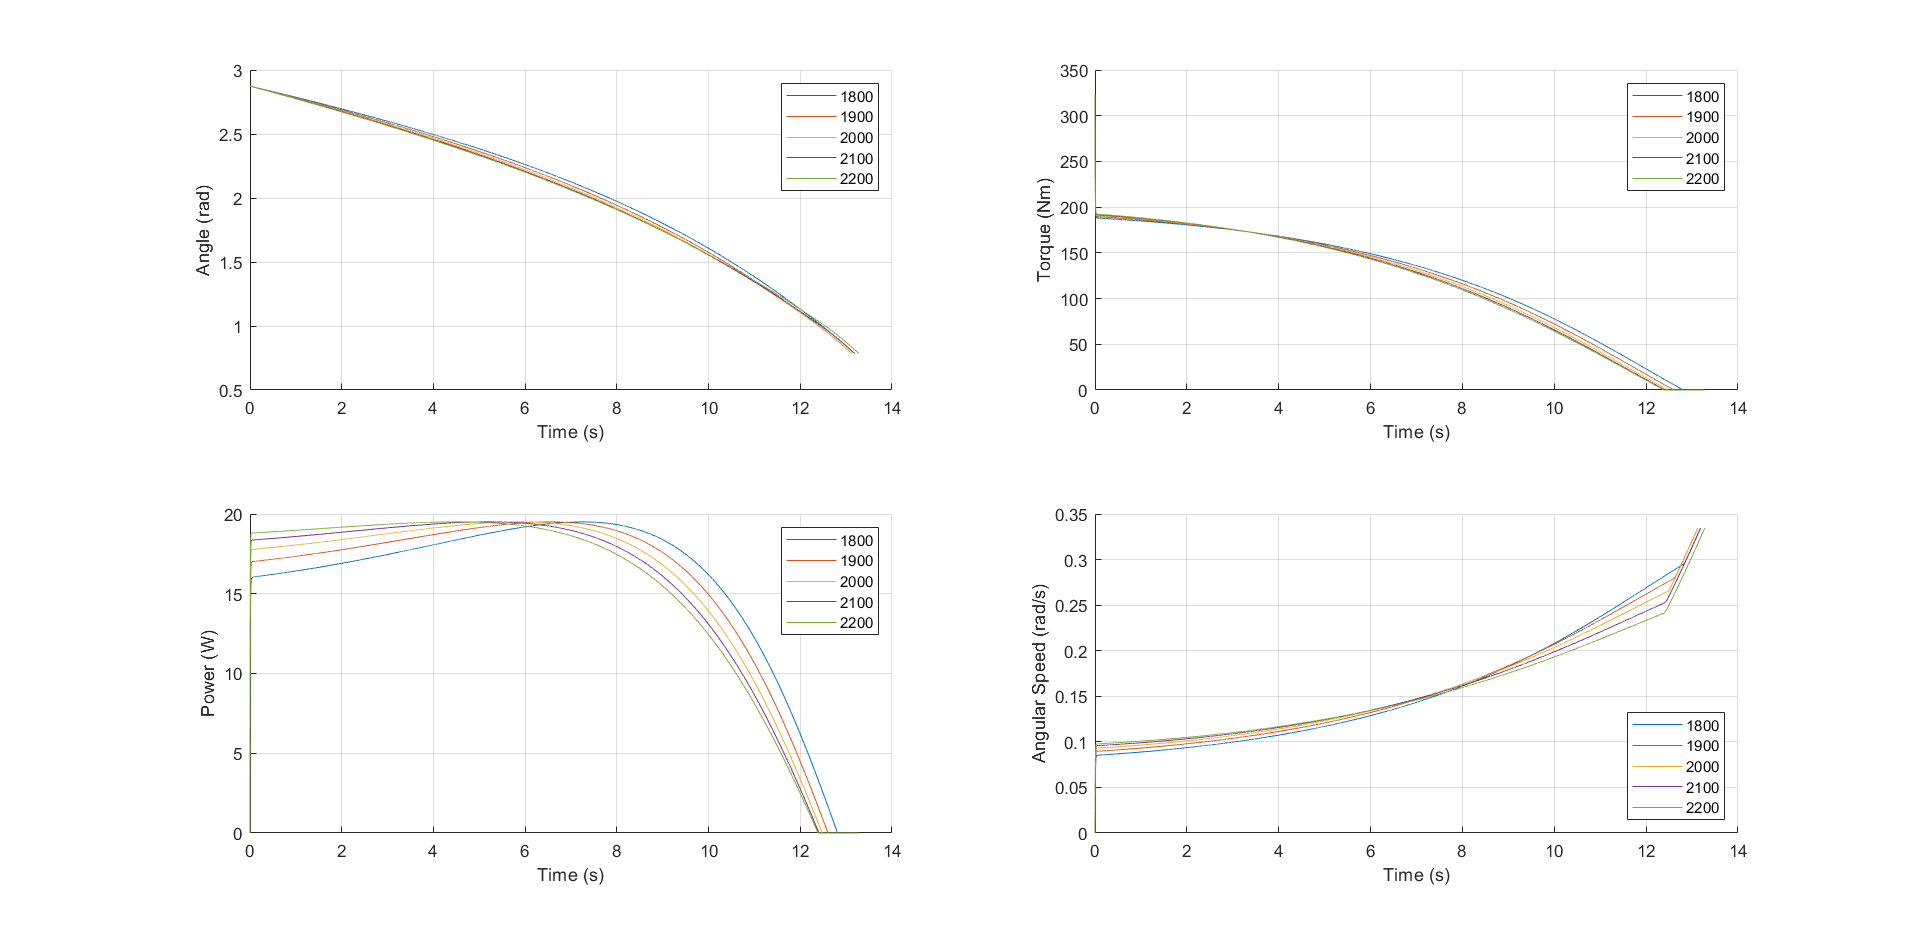
\includegraphics[width=1\textwidth]{Damping_6.png}
    \caption{\label{Damping6} Graphs with damping coefficient of 6}
\end{figure}

\begin{figure}[H]
\centering
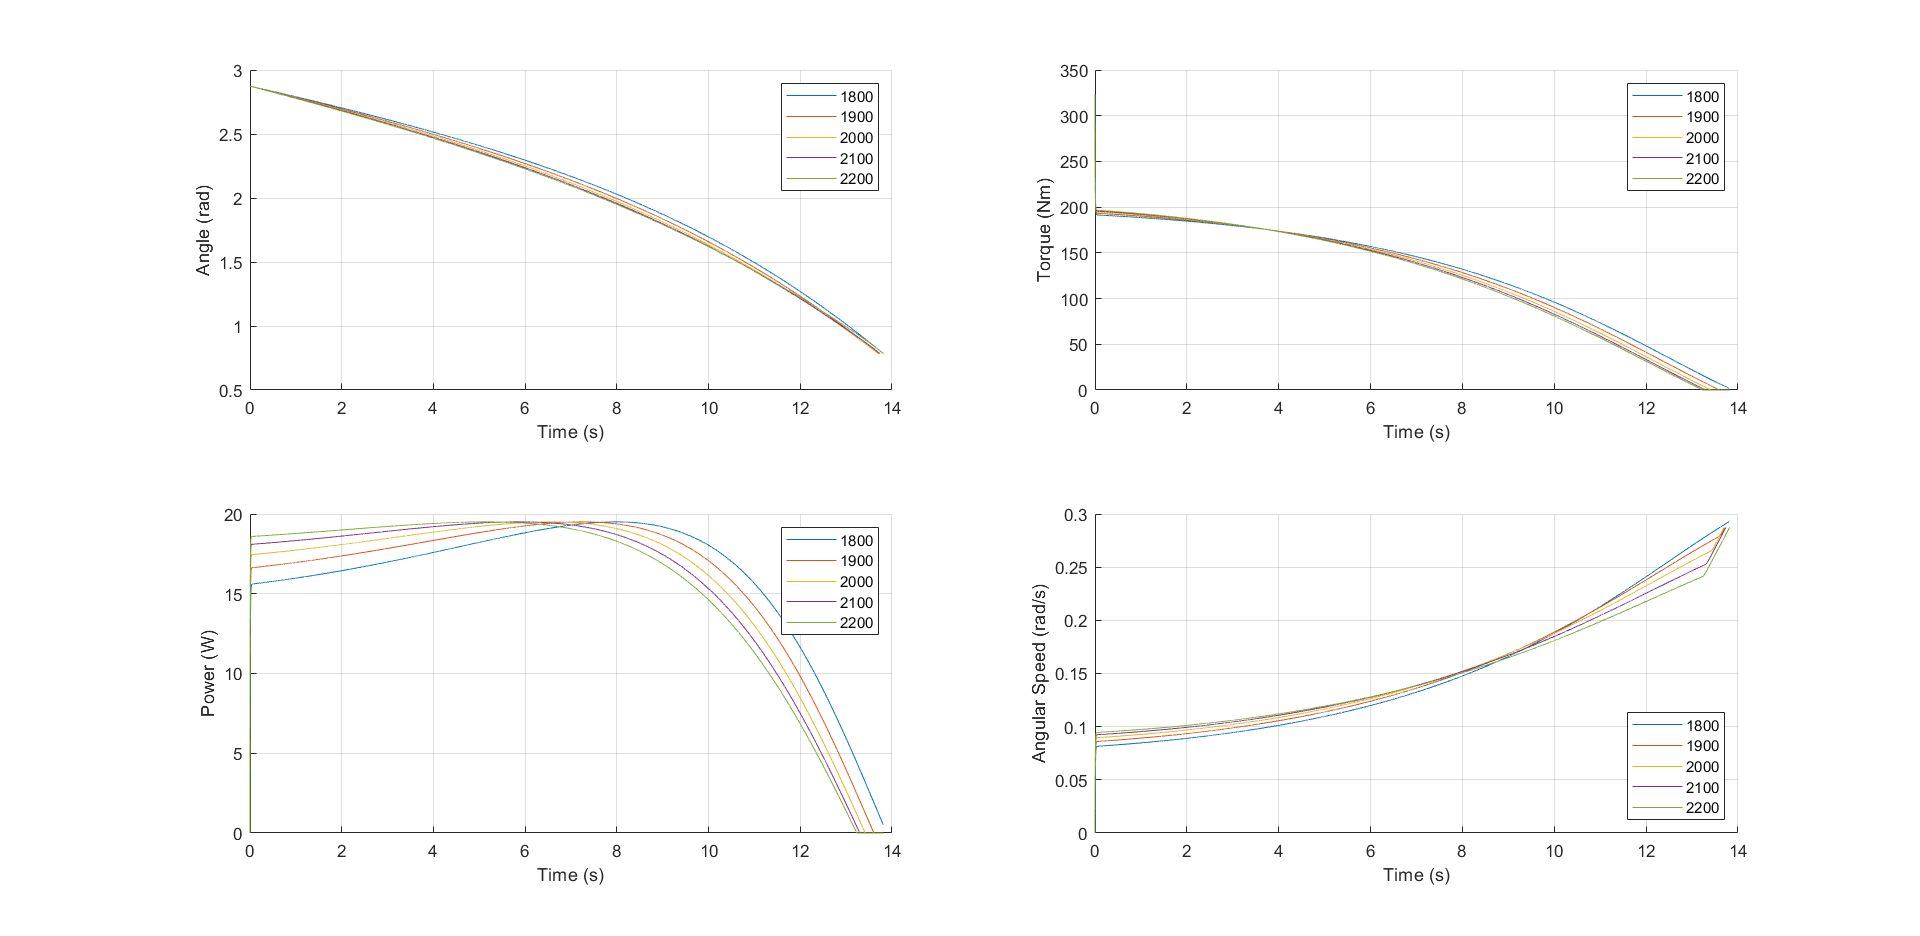
\includegraphics[width=1\textwidth]{Damping_7.png}
    \caption{\label{Damping7} Graphs with damping coefficient of 7}
\end{figure}


It can be seen in figures \ref{Damping4}, \ref{Damping5}, \ref{Damping6}  \& \ref{Damping7} that without a high enough damping coefficient relative to the gear ratio there is a sudden acceleration causing the roof to slam down after the mechanism reaches its highest point. Although this decreases the roof closing time it makes the motion of the roof less aesthetic and has the potential to cause damage. A damping coefficient of 7, shown in Figure \ref{Damping7}, and a gear ratio of 1800 was found to give a smooth curve for angular speed while keeping a deployment time of 13.8 seconds, below the required 15 seconds. This ensured there were no sudden changes in roof speed. The final choice was selected as a gear ratio of 1800 and a damping coefficient of 7 Nm/deg/s as seen in Figure \ref{DFIN}. 

\begin{figure}[H]
\centering
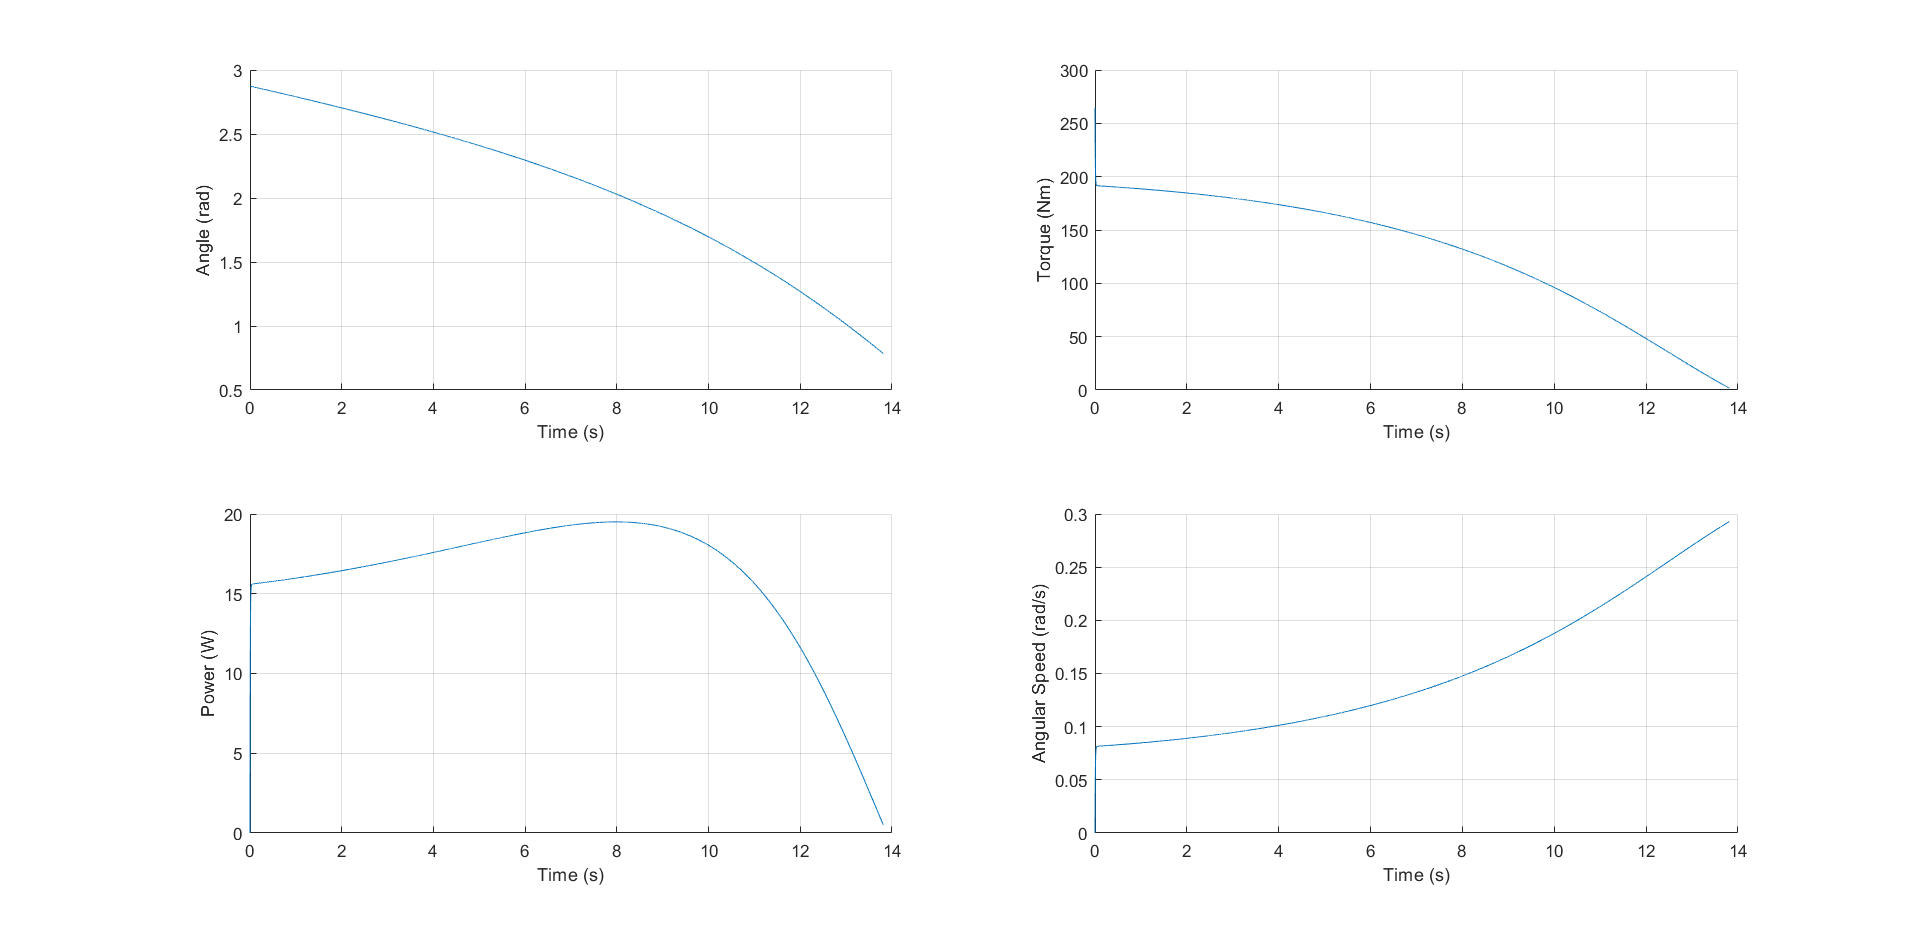
\includegraphics[width=1\textwidth]{Final.png}
    \caption{\label{DFIN} Graphs with damping coefficient of 7 and gear ratio of 1800}
\end{figure}

\section{Multi-stage Gearbox Design}

\begin{table}[H]
\caption{\label{MSG}Multi-stage Gearbox Assesment}
\centering
\begin{tabular}{||c|c|c|c|c|c||}
\hline
Gear stage & 1 & 2 & 3 & 4 & 5 \\ \hline\hline
VR & 5 & 5 & 4.5 & 4 & 4 \\ \hline
Combined VR & 5 & 25 & 112.5 & 450 & 1800 \\ \hline
Module & 1 & 1 & 1 & 1.5 & 1.5 \\ \hline
Pinion teeth & 12 & 12 & 12 & 15 & 15 \\ \hline
Pinion PCD (mm) & 12 & 12 & 12 & 22.5 & 22.5 \\ \hline
Wheel Teeth & 60 & 60 & 54 & 60 & 60 \\ \hline
Wheel PCD (mm) & 60 & 60 & 54 & 90 & 90 \\ \hline
Efficiency & 0.95 & 0.95 & 0.95 & 0.95 & 0.95 \\ \hline
Input Power (W) & 16.7 & 15.87 & 15.07 & 14.32 & 13.60 \\ \hline
Pinion Speed (rpm) & 4000 & 800 & 160 & 35.55 & 8.89 \\ \hline
Wheel Speed (rpm) & 800 & 160 & 35.56 & 8.89 & 2.22 \\ \hline
Pinion Torque (Nm) & 0.04 & 0.19 & 0.90 & 3.86 & 14.66 \\ \hline
Wheel Torque (Nm) & 0.19 & 0.9 & 3.86 & 14.66 & 55.71 \\ \hline
Hunting tooth freq & 800 & 160 & 17.78 & 8.89 & 2.22 \\ \hline\hline
\multicolumn{6}{||c||}{Pinion Forces} \\ \hline
Tangenial Force (N) & 6.67 & 31.67 & 150.42 & 342.95 & 1303.21 \\ \hline
Separating Force (N) & 2.43 & 11.55 & 54.75 & 124.82 & 474.33 \\ \hline
Resultant Force (N) & 7.09 & 33.70 & 160.07 & 364.96 & 1386.85 \\ \hline\hline
\end{tabular}
\end{table}

\paragraph{}
Following the modelling of the mechanism, a multi-stage gearbox was designed to give the designed overall gear ratio and transfer torque from the motor to the mechanism through spur gears. The individual ratios chosen for each step of the gearbox are shown in table \ref{MSG}. Spur gears were chosen as the mechanism is working at low speeds and the loads are not very large. Additionally spur gears are reliable and provide a constant velocity ratio. The gearbox was designed with five stages as spur gears have an upper limit for velocity ratio of 5:1, therefore more stages were required to transmit the torque using the 1800:1 ratio. The velocity ratios selected were used as they provided the overall gear ratio required for the mechanism using simple ratios in the fewest steps. As the efficiency of the pinon and wheel setup is 95$\%$ for each stage the gearbox, using extra steps in the gearbox would result in reduced efficiency of the mechanism and hence influenced our decisions in the design process. The module is found using figure \ref{MSG} from the power at the gearbox stage and the pinon speed. As the power transmitted and pinion speed at the next step is reduced, the module increases for stages 4 and 5. The number of teeth on the pinon and wheel were found from the preferred number of teeth \cite{korane_2015}, and increasing by the velocity ratios. The initial pinion speed, torque and input power were found using the motor specifications shown in Table \ref{IMA}. Using the velocity ratios and efficiency, the wheel speed and torque were calculated. The values for the next steps could then be calculated in a similar way due to the structure of the pinion and wheel gearbox; the pinion for the next step rotates at the same speed as the wheel of the previous step due to being located on the same shaft. The PCD of the pinion and wheel can be calculated using equation \ref{M}, where M is the Module, D is the PCD in millimetres and N is the number of teeth on the spur gear.

\begin{equation}
    M=D/N
    \label{M}
\end{equation}

The tangential and separating forces on the gears can be found by assuming a pitch angle ($\theta$) of 20$^{\circ}$ for spur gears using equations \ref{M} and \ref{Ft} respectively. 

\begin{equation}
    F_{t}=2 T/d
    \label{Ft}
\end{equation}

The tangential force, equation \ref{Ft}, is calculated from the pinion torque (T) and PCD of the pinion (d). 

\begin{equation}
    F_{s}=F_{t} tan(\theta)
    \label{Fs}
\end{equation}

The separating force, equation \ref{Fs}, is calculated by multiplying the tangential force and the tangent of theta. The resultant force on the spur gear teeth is found using  equation \ref{F}.

\begin{equation}
    F = \sqrt{F_t^2 + F_s^2}
    \label{F}
\end{equation}

\section{Solution Specification}

The Solution Specification (Table \ref{SolSpec}) shows the final values from the analysis in comparison to the initial PDS. It was found that the final feasible design was successfully able to achieve all of the Must requirements in the PDS and most of the Wish requirements. The crash safety legislation for roll over was unable to be evaluated at this stage of the design process and hence this factor could not be judged.

\begin{table}[H]
\centering
\caption{Solution Specification}
\label{SolSpec}
\begin{tabular}{||l|l|l|l||}
\hline
Category & Requirement & PDS No. & Value \\
\hline\hline
\multirow{5}{*}{Motor} & Selection & 7 & 0 130 001 001 \\ \cline{2-4} 
 & Required Voltage & 8 & 12 V \\ \cline{2-4} 
 & Efficiency & 17 & 77\% \\ \cline{2-4} 
 & Max Torque & 3 & 159.20 Nm \\ \cline{2-4} 
 & Min Torque & 3 & 0 Nm \\ \hline
\multirow{2}{*}{Gearbox} & Gear ratio & 2,3 & 1800 : 1 \\ \cline{2-4} 
 & Selection & 2,3 & 5:1, 5:1, 4.5:1, 4:1, 4:1 \\ \hline
Damper & Coefficient & 20 & 7 Nm/deg/s \\ \hline
\multirow{3}{*}{Roof and Mechanism} & Deployment Time & 2,20 & 13.8 s \\ \cline{2-4} 
 & Material & 4 & Canvas and Butyl Rubber \\ \cline{2-4} 
 & Mass & 4 & 31.7 kg \\ \hline\hline
\end{tabular}
\end{table}

\section{Conclusion}
In this project, concepts for mechanisms were generated and compared against each other in order to determine the most suitable. The selected mechanism was then modelled and refined in order to perfectly fit the requirements stated in the PDS Table \ref{PDS}. A motor, gear ratio and damping constant were then selected in order to obtain suitable values for output torque and speed of rotation for the desired deployment time. The ideal values for these were then selected and a gearbox configuration and forces calculated to give a gear ratio of 1800 : 1 and maximum output torque as 159.2 Nm. It was found that the mechanism was a feasible design which created an ideal balance between the categories stated in the PDS. The project achieved a suitable working roof mechanism which closed in 13.8 seconds whilst forming an aesthetically shaped structurally sound arch.

\paragraph{}
In future, worm gears could be investigated to replace the spur gears in the gearbox. Using worm gears would increase the velocity ratio required to transmit the torque for the mechanism, reducing the number of stages in the gearbox and therefore saving space in the car. However this would also further decrease the efficiency of the gearbox compared to spur or helical gears. Additionally, if the project was progressed further, the beam dimensions would be refined to better analyse the bending stresses caused by the weight of the roof and window. During the project the mechanism was designed and modelled in a 2D profile, whilst future analysis would be carried out for the mechanism in 3D to give a more accurate representation. The mechanism designed did not include the mounting of the roof mechanism onto the windscreen or the specification for the bearings in the mechanisms; this would be required if the concept was taken to production. Another further step would be to add a reverse gear allowing the roof to be retracted. This would further decrease the efficiency of the gearbox, slowing the retraction time down as the motor torque value would need to be increased.

\bibliographystyle{plain}
\bibliography{References}

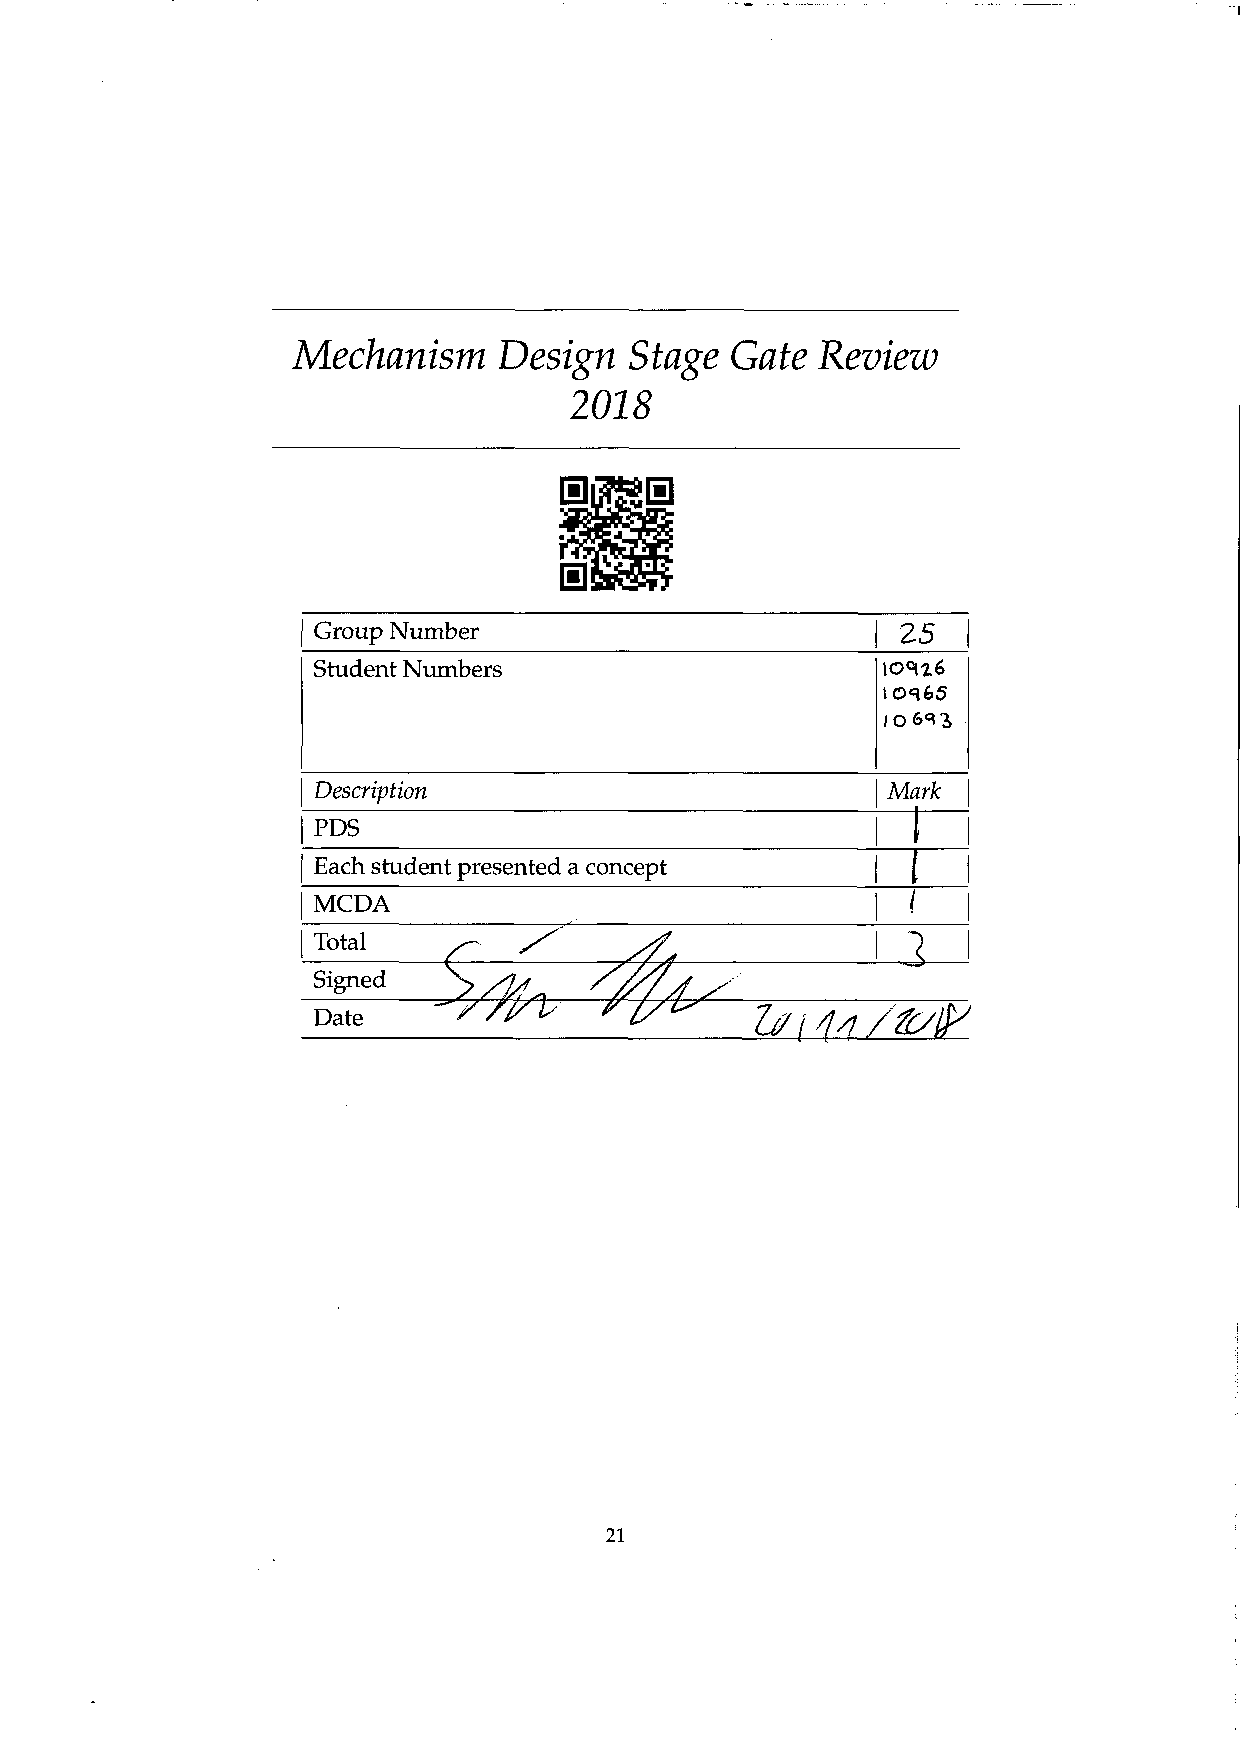
\includepdf[pages=-]{Review}

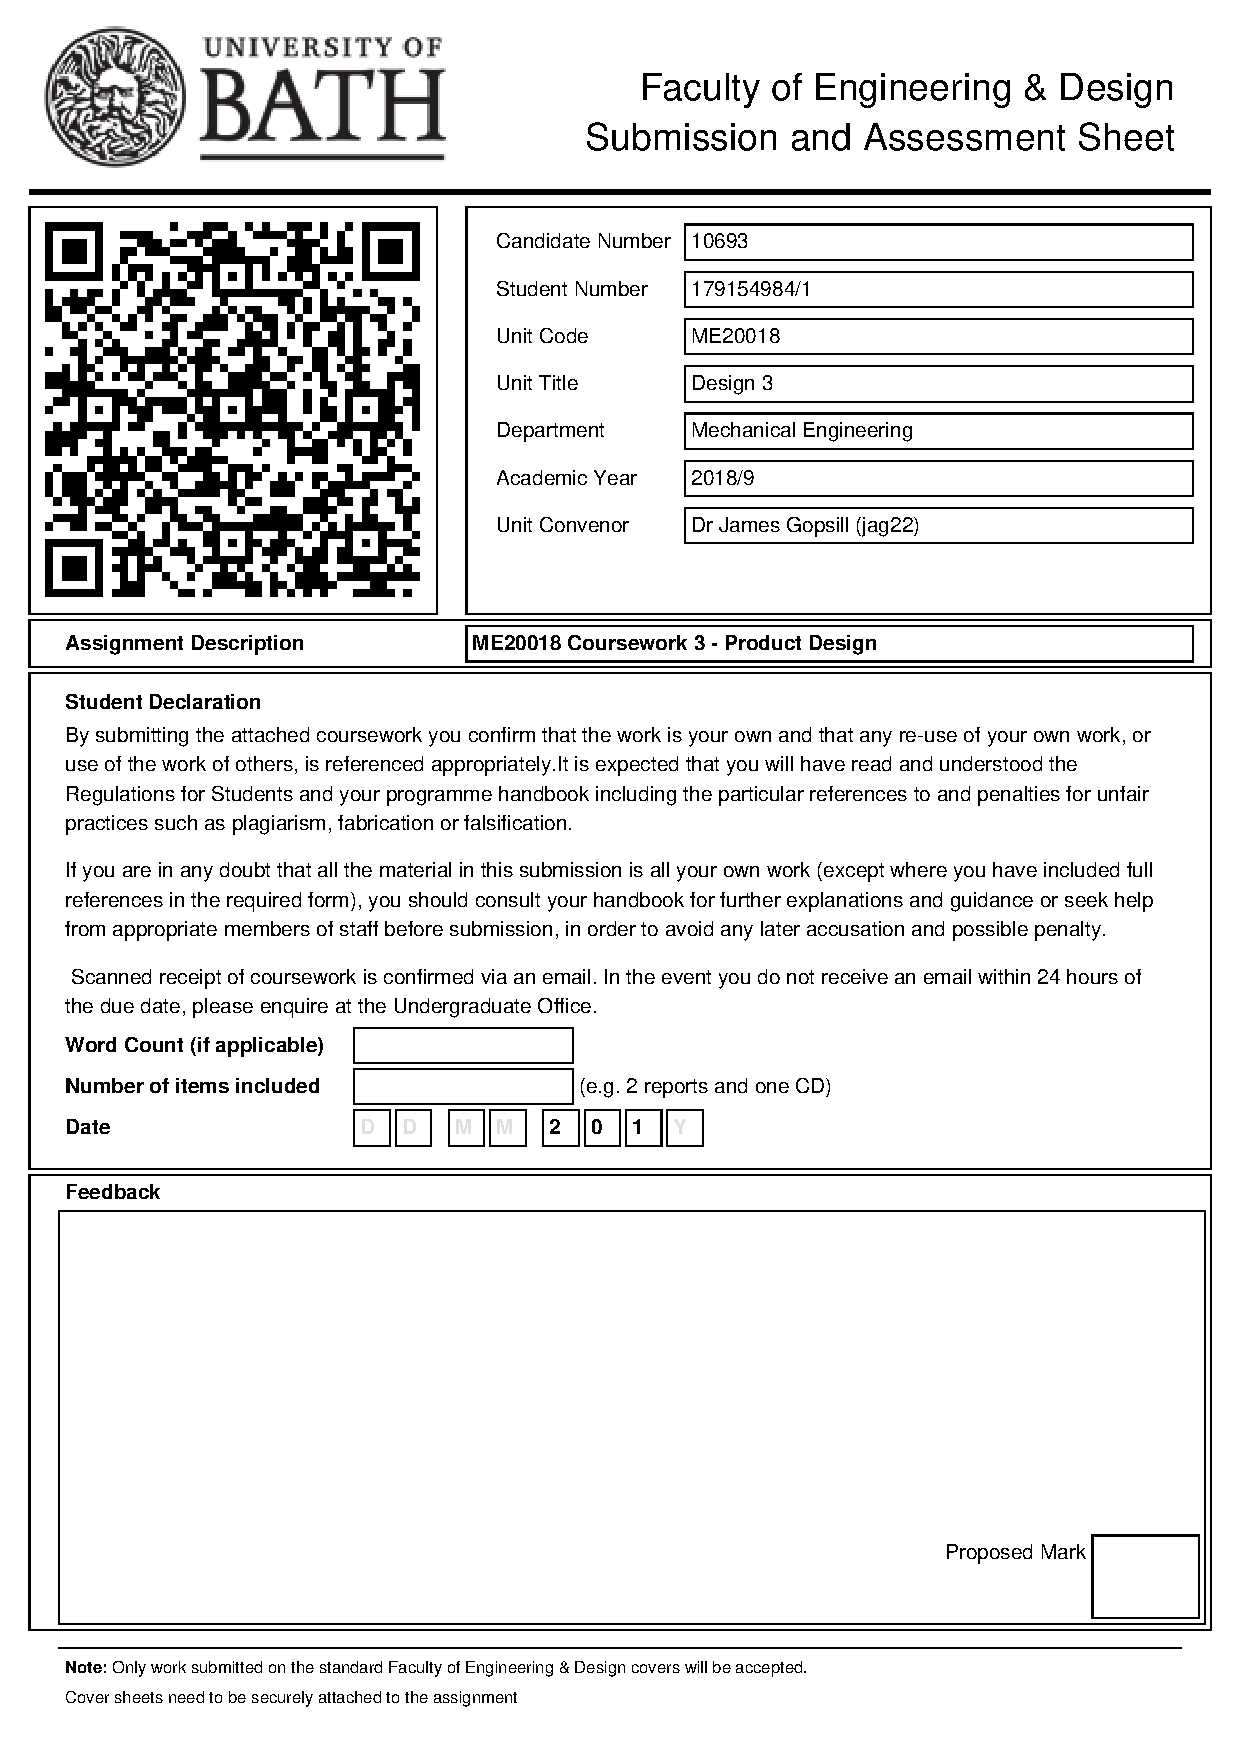
\includepdf[pages=-]{StuartCoversheet}
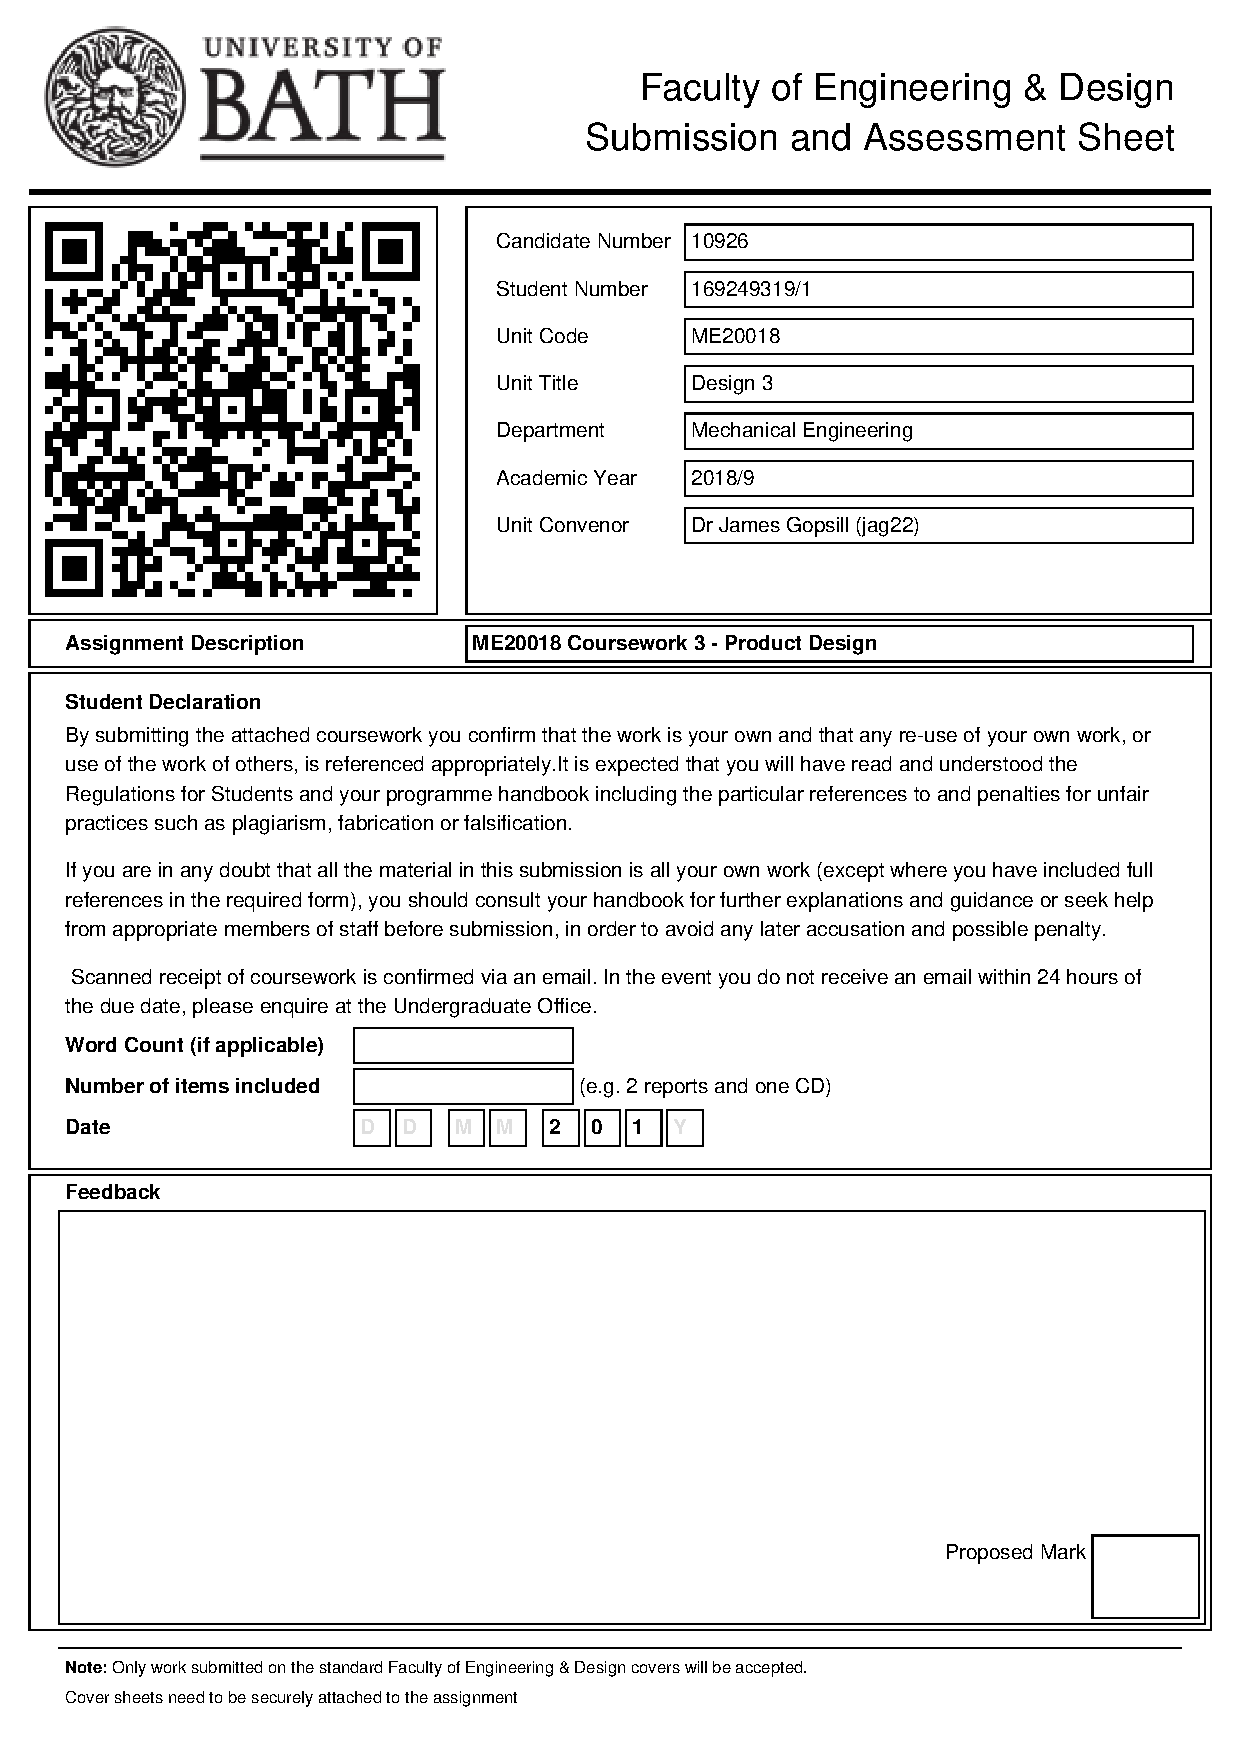
\includepdf[pages=-]{FabianCoversheet}
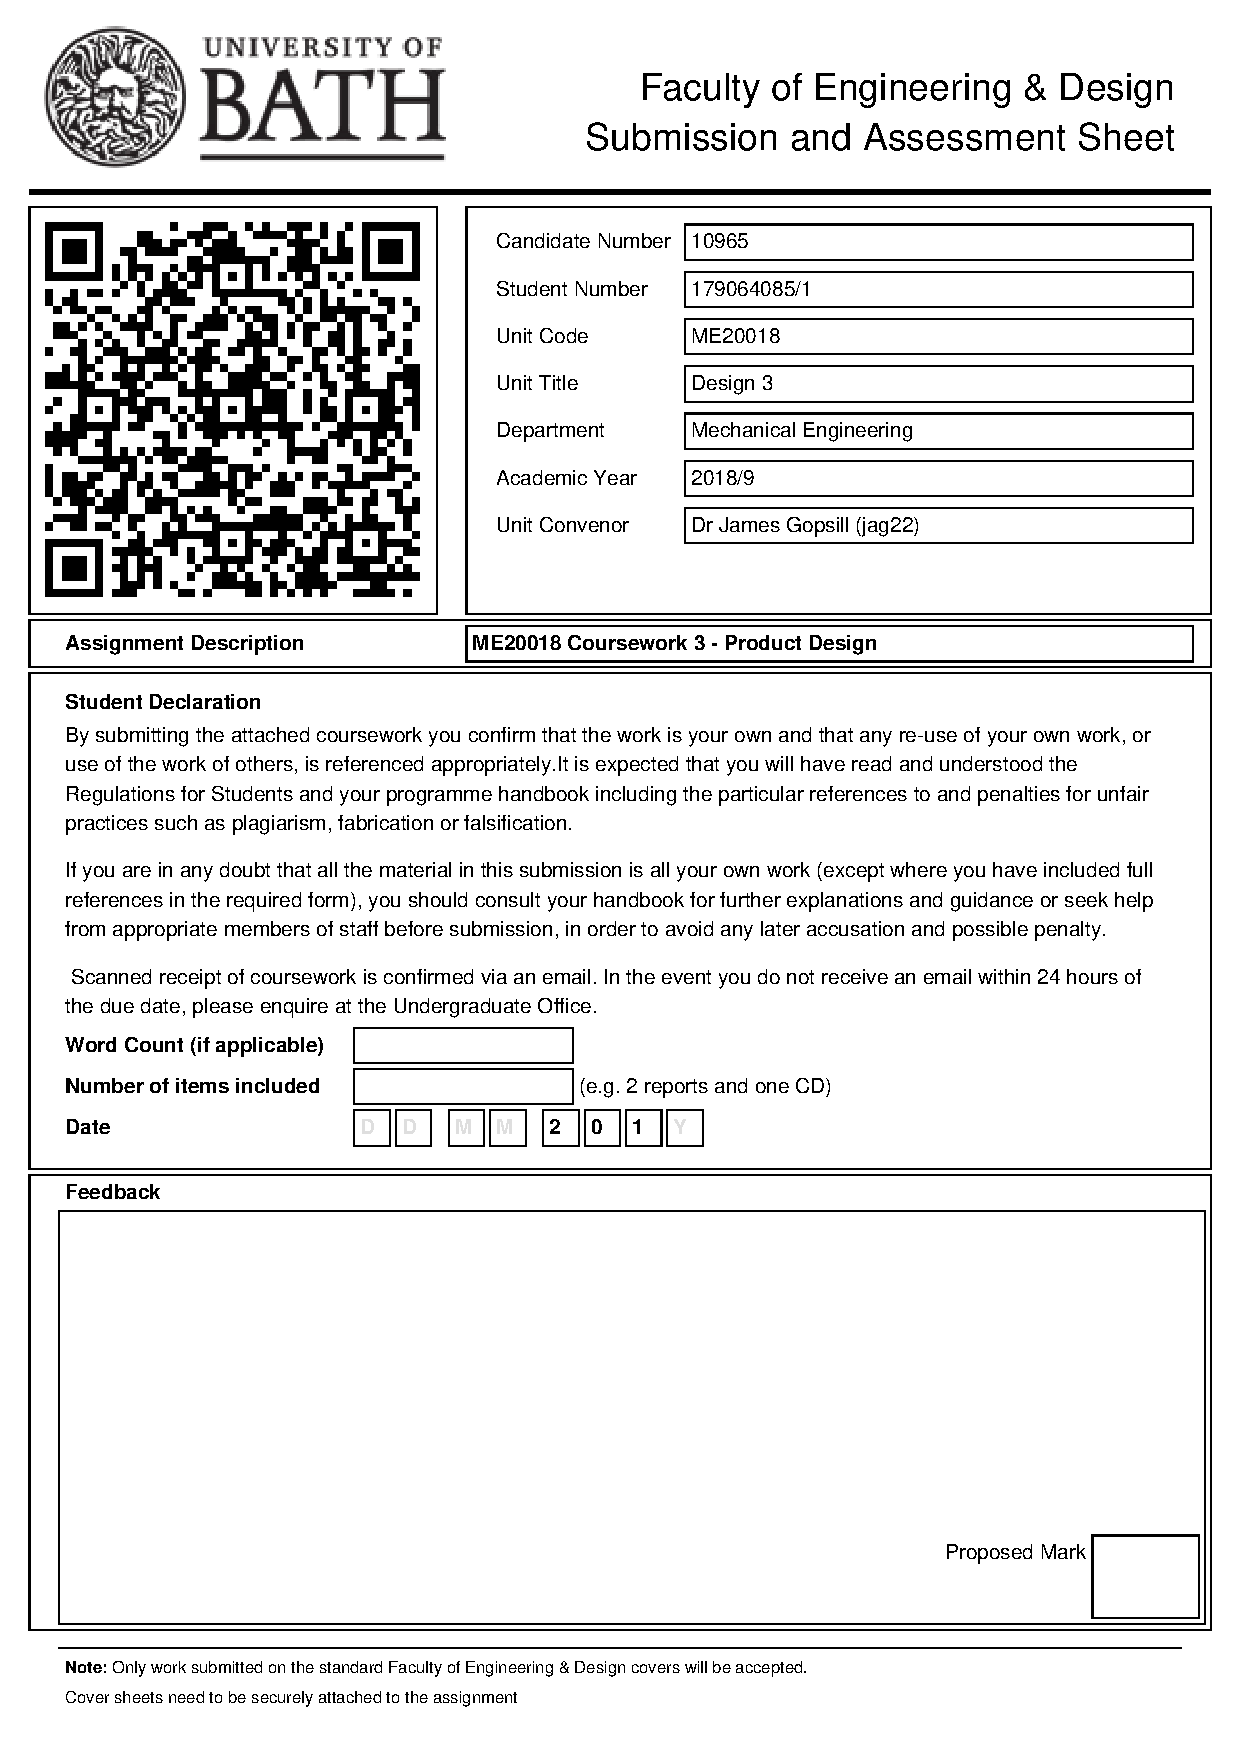
\includepdf[pages=-]{TerryCoversheet}

\end{document}